\documentclass[10pt, titlepage]{amsart}
\usepackage[a4paper, total={6in, 8in}]{geometry}

\usepackage{amsmath, amsthm, ulem, graphicx, marvosym, fancyhdr, amscd, amssymb, enumitem, mathrsfs, multicol, setspace}
\usepackage{enumitem}
\usepackage{booktabs}
\usepackage{listings}             % Include the listings-package
\usepackage{seqsplit}
\usepackage{cleveref}
\usepackage[table,xcdraw]{xcolor}
\usepackage{amsaddr}

\newcommand\Z{{\mathbb Z}}
\newcommand\F{{\mathbb F}}
\newcommand\N{{\mathbb N}}
\newcommand\A{{\mathbf A}}
\newcommand\p{{\mathscr P}}
\newcommand\R{{\mathbb R}}
\newcommand\Q{{\mathbb Q}}
\newcommand\C{{\mathbb C}}
\newcommand\bfx{{\mathbf x}}
\newcommand\bfv{{\mathbf v}}
\newcommand\bfy{{\mathbf y}}
\newcommand\bfw{{\mathbf w}}

%\usepackage{graphics}

%\topmargin -.7in
%\evensidemargin-0in
%\oddsidemargin0in
%\textheight 9.5in
%\textwidth 6.5in

%\def\arraystretch{1.5}%  1 is the default, change whatever you need

\newtheorem{theorem}{Theorem}[subsection]
\newtheorem{lemma}{Lemma}[subsection]
\newtheorem{prop}{Proposition}[subsection]
\newtheorem{cor}{Corollary}[subsection]
\newtheorem{algorithm}{Algorithm}[subsection]
\theoremstyle{definition}
%\newtheorem{defi}{Definition}[subsection]
\newtheorem{definition}{Definition}[subsection]
\newtheorem{example}{Example}[subsection]
\newtheorem{rmk}{Remark}[subsection]
\newtheorem{interpret}{Interpretation}[subsection]
%\theoremstyle{test}
\newtheorem*{axioms}{Axioms}

%\everymath={\displaystyle}

\pagestyle{headings}
%\onehalfspacing

\title{Testing for Compositeness}
\author{Miguel Amezola %\\
%	B.S. Mathematics \\
%	Pacific Lutheran University  \\
%	Advisors: Dr. Tom Edgar
	%	\and
	%	Your friend who worked with you \\
	%	His/her Major / University \\
}
\address{	B.S. Mathematics \\
	Pacific Lutheran University  \\
	Advisors: Dr. Tom Edgar}
\email{math@miguelamezola.com}

\date{\today}

\setcounter{secnumdepth}{2}


\begin{document}
	
	\lstset{language=Python}          % Set your language (you can change the language for each code-block optionally)
		
	%\thispagestyle{empty}
	
	\begin{abstract}
		The problem of distinguishing composite numbers from primes is an important task for mathematicians and many others.
		We explore two methods for performing such a binary classification of the integers.		
		We begin with the mathematical formulation of a classic test for compositeness known as the Miller-Rabin test.
		This involves the exposition of concepts from number theory, such as divisibility and modular arithmetic, and algebraic structures like monoids, groups, and rings.
		We follow this with an evaluation of Miller-Rabin's performance in comparison with a modern machine learning algorithm called Support Vector Machine.
	\end{abstract}

	\maketitle
	
	\tableofcontents
	\newpage
	
	% ==========================================================================
	% Intro
	% ==========================================================================		
	
	\section{Introduction}
	Johann Carl Friedrich Gauss once wrote that ``the problem of distinguishing prime numbers from composite numbers \ldots is known to be one of the most important and useful in arithmetic \ldots Further, the dignity of the science itself seems to require that every possible means be explored for the solution of a problem so elegant and so celebrated."\cite{gauss}
	In this spirit, we will explore two methods for the binary classification of integers as either prime or composite. 

%		Machines have displayed a significant level of learning ability. But how well can a machine learn a primality test from the integer sequence associated with it?

		
	%\subsection{Prime and Composite Numbers}
	
	%All integers greater than one are either prime or composite. 
	We formally define these mutually exclusive classes of integers as follows.
	\begin{definition}[Prime]\label{definition:prime}
		Let $p \in \Z$, $p > 1$. Then $p$ is prime if and only if for every $a, b \in \Z$, $p=ab$ implies $a=1$ or $b=1$. \cite{pommersheim}
	\end{definition}
	\begin{definition}[Composite]\label{definition:composite}
		Let $n \in \Z, n > 1$. Then $n$ is composite if and only if there exists $a, b \in \Z$ such that $n=ab, 1<a,b<n$. \cite{pommersheim}
	\end{definition}
	
	Of course, all even integers greater than 2 are composite since they are all multiples of 2. Likewise, every multiple of 5 or 10 is composite. For relatively small integers, the existence of $a, b \in \Z$ such that $n=ab$ with $1<a,b<n$ is easy to establish. For example, $63$ is composite since $63 = 9 \cdot 7$ and $1023$ is composite since $1023 = 341 \cdot 3$. 
	
	We notice that both $63$ and $1023$ have factors less than their squared roots; that is, $7 < \sqrt{63} \approx 7.94$ and $3 < \sqrt{1023} \approx 31.98$. Suppose that this is not true for some composite number $n = ab$. Then $a,b \geq \sqrt{n}$. But this leads to a contradiction, $n = ab > \sqrt{n} \cdot \sqrt{n} = n$ but $n$ cannot be greater than itself. Thus, either $a < \sqrt{n}$ or $b < \sqrt{n}$. 
	
	%Since every integer greater than or equal to 2 has a prime factor, any such factor of $a$ or $b$ is also a factor of $ab = n$. Hence, every composite number $n$ has a prime factor $p$ such that $p < \sqrt{n}$.
	
	This fact is used in a common test for compositeness called trial division. For instance, suppose that we would like to know whether or not 201 is composite. We know that $\sqrt{201} \approx 14.18$ and so we only have to check if $201$ is a multiple of $2, 3, 4, \ldots, 14$. Since 201 is not even, we know that it is not a multiple of $2$ and so we proceed with the next integer. We then discover, to our delight, that $201 = 3 \cdot 67$. Hence, 201 is composite. 
	
	Unfortunately, trial division is a laborious task for large integers like 154,320,140,719,313. The square root of this number is 12,422,566. That means that we would have to check whether or not any integer between 2 and 12,422,566 is a multiple of 154,320,140,719,313. Even if we noticed that every integer greater than or equal to 2 has a prime factor, and that any factor of $a$ or $b$ is also a factor of $ab = n$, and so every composite number $n$ has a prime factor $p$ such that $p < \sqrt{n}$, we would still have to perform trial division for 154,320,140,719,313 with every prime between 2 and its first prime factor 349! 
	
	For this reason, we would like to explore more efficient compositeness tests. First, we will consider a classic algorithm known as the Miller-Rabin test, followed by a method that uses a modern machine learning algorithm called a Support Vector Machine. However, before we are ready to do so, we must discuss the concepts in number theory and abstract algebra that form the foundation of the Miller-Rabin test.
	
	\section{Background for the Miller-Rabin Test}
	
	\subsection{Divisibility}
	Divisibility is a key concept in number theory.
	%The Miller-Rabin test uses modular arithmetic. 
	The Miller-Rabin test uses two key facts related to divisibility, namely,
	\begin{enumerate}
		\item two integers with a greatest common divisor equal to 1 are relatively prime, and 
		\item the greatest common divisor of two integers is the smallest possible linear combination of those integers. 
	\end{enumerate}
	Both facts rely on the following definition.
		
	\begin{definition}[Divide]\label{definition:divide}
		Let $a,d \in \Z$. We say that $d$ divides $a$ if there exists $q \in \Z$ such that $a = qd$. We express this in symbols as $d \mid a$ (which is read ``$d$ divides $a$"). We refer to $d$ as a divisor of $a$. \cite{pommersheim}
	\end{definition}
	
	In our discussion regarding composite numbers, we concluded that $63$ is composite since $63 = 9 \cdot 7$ and $1023$ is composite since $1023 = 341 \cdot 3$. Thus, according to this definition, we can say that 7 divides 63 and 341 divides 1023. However, like most composite numbers, 63 and 1023 have more divisors, i.e. $1, 3, 7, 9, 21, 63$ divide $63$ and $1, 3, 11, 31, 33, 93, 341, 1023$ divide $1023$. Notice that the greatest number in both lists is $3$. This is their greatest common divisor.
	
	% two integers with a greatest common divisor equal to 1 are relatively prime

	\begin{definition}[Greatest common divisor]\label{definition:gcd}
		Let $a,b \in \Z$ be nonzero. The greatest common divisor of $a$ and $b$ is the largest $d \in \N$ for which $d \mid a$ and $d \mid b$ and is denoted $d = \gcd(a,b)$.
	\end{definition}		

%	\begin{example}
%		The divisors of $42$ are $1,2,3,6,7,14,21,42$ and the divisors of $49$ are $1,7,49$. The largest number that appears in both of these lists is $7$. Thus, $7 = \gcd(42,49)$.
%	\end{example}
	
	However, the greatest common divisor of some integers is $1$. For instance, the divisors of $25$ are $1,5,15$ and the divisors of $28$ are $1,2,4,7,14,28$. The largest number that appears in both lists is $1$, and so $\gcd(25, 28) = 1$. Such numbers are said to be relatively prime.
	
	\begin{definition}[Relatively prime]\label{definition:relatively_prime}
		Let $a, b \in \Z$. We say $a$ and $b$ are relatively prime if $\gcd(a,b)=1$. 
	\end{definition}
	
	\begin{prop}\label{prop:gcd_is_1}
		Let $a, p \in \Z$ such that $p$ is prime and $p \nmid a$, then $\gcd(a,p) = 1$.
	\end{prop}
	
	\begin{proof}
		We will use contradiction. 
		Let $a, p \in \Z$ such that $p$ is prime and $p \nmid a$. 
		Suppose $\gcd(a,p) \neq 1$, then $a = kd$ and $p = ld$ for some $d,k,l \in \Z$ with $d \neq 1$.
		Since $p$ is prime and $d \neq 1$, then $l=1$ and $d=p$ by \cref{definition:prime}.
		But $a=kd=kp$ if and only if $p \mid a$, contradicting the fact that $p \nmid a$.
		Therefore, we must conclude that $\gcd(a,p) = 1$.
	\end{proof}
	
	% the greatest common divisor of two integers is the smallest possible linear combination of those integers

	Hence, two integers with a greatest common divisor equal to 1 are relatively prime. In particular, a prime number is relatively prime to any integer that it does not divide. Lastly, we will show that the greatest common divisor of two integers is the smallest possible linear combination of those integers.
				
	\begin{lemma}[Linear combination]\label{lemma:linear_combination}
		Let $d,m,n,x,y \in \Z$. If $d \mid x$ and $d \mid y$, then $d \mid mx + ny$.
	\end{lemma}
	
	\begin{proof}
		Let $d,m,n,x,y \in \Z$ such that $d \mid x$ and $d \mid y$.
		Since $d \mid x$, then there exists $k \in \Z$ such that $x = kd$.
		Multiplying by $m$, we have  $mx = mkd$.
		Since $d \mid y$, then there exists $l \in \Z$ such that $y = ld$.
		Multiplying by $n$, we have  $ny = nld$.
		Adding both results yields $$ mx + ny = mkd + nld = (mk+nl)d.$$
		Therefore, since $(mk+nl) \in \Z$, we know $d \mid mx + ny$.
	\end{proof}
	
	\begin{prop}\label{proposition:smallest_possible_linear_combination}
		Let $a,b \in \Z$. Then greatest common divisor of $a$ and $b$ is equal to the smallest positive linear combination of $a$ and $b$.
	\end{prop}
	
	\begin{proof}
		We will use contradiction.
		Let $a,b \in \Z$, and suppose $e=ax+by$ is the smallest positive linear combination of $a$ and $b$.
		Let $d = \gcd(a,b)$. Then $d \mid a$ and $d \mid b$ implies that $d \mid ax + ay$ by 		\cref{lemma:linear_combination}.
		Since $d \mid ax+by$, then $d \mid e$, and so $d \leq e$.
		
		Now suppose $e \nmid a$. Thus, $a = qe + r$ for some $q \in \Z$ with $0 < r < e$. Then 
		$$r = a-qe = a-q(ax-by) = a-qax-qby = a(1-qx)- b(qy).$$
		This means that $r$ is a positive linear combination that is less than $e$, contradicting the fact that $e$ is the smallest positive linear combination of $a$ and $b$. Hence, $e \mid a$, and a similar argument can be used to show that $e \mid b$ as well. Thus, by \cref{lemma:linear_combination}, $e \mid d$ and $e \mid ax + by$, and so $e \leq d$.
		
		Since we have $d \leq e$ and $e \leq d$, it must be the case that $e=d$. Therefore, the greatest common divisor of $a$ and $b$ is equal to the smallest positive linear combination of $a$ and $b$.
	\end{proof}

	
	% ==========================================================================
	% Congrunces
	% ==========================================================================	
	\subsection{The Set of All Congruence Classes}
	
	Divisibility can be used to partition the set of all integers into a finite number of classes. 
	These classes are groups of integers with a common property related to the following definition.
	%The following equivalence relation is used to define these classes.
	
%	\begin{lemma}\label{lemma:divisibility}
%		Let $a, d \in \Z: a, d \geq 1$. If $d | a$, then $1 \leq d \leq a$. \cite{pommersheim}
%	\end{lemma}
%	
%	\begin{proof}
%		Let $a, d \in \Z: a, d \geq 1$ such that $d | a$. By \cref{definition:divisibility}, $\exists q \in \Z : a = qd$ since $d | a$. Furthermore, it must be that $q \geq 1$ and $d \geq 1$ so that $qd = a \geq 1$. Hence, $1 \leq d \leq qd = a$. Therefore, $1 \leq d \leq a$.
%	\end{proof}
%	
	
	\begin{definition}[Congruent]\label{definition:congruent}
		Let $a,b,n \in \Z$ with $n > 0$. We say that $a$ is congruent to $b$ modulo $n$ if $n \mid (a - b)$, denoted $a \equiv b \pmod n$. \cite{pommersheim}
	\end{definition}
	
%	Notice that every integer that is a multiple of $-1$ is also a multiple of $1$. Thus for instance $-1 | 5 - 3$ since $5-3 = 2 = -2(-1)$ and $1 | 5 - 3$ since $5-3 = 2 = 2(1)$. Therefore, $5$ and $3$ are congruent modulo $-1$ and modulo $1$. The same is true for $-54$ and $54$ because $120 - 12 = 108 = -2(-54)$ and $120 - 12 = 108 = 2(54)$; that is, $120$ and $12$ are congruent modulo $-54$ and modulo $54$. Hence, we will 
%	
%	\begin{prop}
%		Congruence is an equivalence relation.
%	\end{prop}
%	
%	\begin{proof}
%		Let $a,b,c,n \in \Z, n>0$. Since $0 = 0 \cdot n$, we know $n \mid 0$. Then $n \mid 0 = n \mid a-a$ if and only if $a \equiv a \pmod n$. Thus, congruence is reflexive. To show that it is also symmetric, suppose $a \equiv b \pmod n$. Notice that $n \mid p \iff p = qn \iff -p = -qn \iff n \mid -p$. Hence, $n$ divides both $q$ and $-q$. Thus, $a \equiv b \pmod m \iff n \mid a - b \iff n \mid -(a-b) = n \mid b-a \iff b \equiv a \pmod n$, and so congruence is symmetric. Lastly, we must show transitivity. So, assume $a \equiv b \pmod n$ and $b \equiv c \pmod n$. This means that $n$ divides both $a-b$ and $b-c$. Then, by \cref{definition:divisibility}, $a-b = kn$ and $b-c = ln$ for some $k,l \in \Z$. Adding these we have $a-c = a-b+b-c = (a-b)+(b-c) = kn + ln = (k+l)n$; that is, $a-c = (k+l)n$, which implies that $n$ divides $a-c$. Therefore, $a \equiv c \pmod n$, and so we have proven transitivity.
%	\end{proof}
	
	\begin{prop}\label{proposition:equivalent_conditions_for_congruent}
		Let $a, b, n \in \Z$. Then the following conditions are all equivalent.
		\begin{enumerate}
			\item $a = b + kn$ for some $k \in \Z$;
			\item $n \mid a - b$;
			\item $a \equiv b \pmod n$.
		\end{enumerate}		
	\end{prop}
	
	\begin{proof}
		Let $a, b, n \in \Z$.
		First suppose condition (1).
		Then $a = b + kn$ implies $a-b = kn$.
		By the definition of divide, it follows that $n \mid a - b$.
		Thus, condition (1) implies condition (2).
		
		Now suppose condition (2).
		Then, by the definition of congruent, $n \mid a - b$ implies $a \equiv b \pmod n$.
		Therefore, condition (2) implies condition (3).
		
		Finally, we would like to show that condition (3) implies condition (1).
		So, we assume $a \equiv b \pmod n$.
		Then, by the definition of congruent, we know $n \mid a - b$.
		If follows that there exists $k \in \Z$ such that $a-b = kn$ by the definition of divide.
		Therefore, condition (3) implies condition (1).

	\end{proof}
	
	% Which integers are also congruent to $144$?
	
%	\begin{theorem}[Equivalent Conditions for Congruence]\label{theorem:equivalent_conditions_for_congruence}
%		Let $a, b \in \Z, n \in \N$. The following statements are equivalent:
%		\begin{enumerate}
%			\item $a \equiv b \pmod b$
%			\item $n \mid (a - b)$
%			\item $\exists k \in \Z$ such that $a = b + kn$
%			\item when $a$ and $b$ are divided by $n$, they leave the same remainder.
%		\end{enumerate} \cite{pommersheim}
%	\end{theorem}
%	
	\begin{example}\label{example:congruent}
		Let $a = 34$, let $b = 144$, and let $n = 10$. Since $34 - 144 = -110 = -11 \cdot 10$, we have
		\begin{enumerate}
			\item $34 = 144 + (-11) \cdot 10$,
			\item $10 \mid 34 - 144$, and
			\item $34 \equiv 144 \pmod{10}$
		\end{enumerate}
		as expected.
	\end{example}
	
	However, 34 is not the only integer that is congruent to 4 modulo 10. In fact, every integer 4 more than a multiple of 10 also shares this property. This set of integers is an example of what we will call a congruence class.


	\begin{definition}[Congruence Class]\label{definition:congruence_class}
%		Let $n \in \N$, and let $b \in \Z$. Then the \textbf{congruence class} of $b$ modulo $n$ is the set of all integers congruent to $b$ modulo $n$: $$ \bar{b} := \{ x \in \Z : x \equiv b \pmod n \}. $$ The congruence class of $b$ modulo $n$ may also be defined as $$ \bar{b} := \{ b + kn : k \in \Z \}. $$
		Let $a,n \in \Z$ with $n > 0$. We define the congruence class of $a$ modulo $n$ as the set of all integers congruent to $a$ modulo $n$; that is, $$\bar{a} := \{ x \in \Z : x \equiv a \pmod n \}.$$% $$ \bar{a} := \{ a + kn : k \in \Z \}.$$
	\end{definition}
	
	Each modulus partitions the entire set of integers into finitely many congruence classes. 
	\begin{example}
		Let $n=3$. Then $\bar{0} \in \Z_3$ contains all the multiples of 3, $\bar{1} \in \Z_3$ contains all the integers that are 1 more than a multiple of 3, and $\bar{2} \in \Z_3$ contains all the integers that are 2 more than an multiple of 3. However, integers that are congruent to 4 modulo 3 are equal to $1 + k \cdot 3$ according to \cref{proposition:equivalent_conditions_for_congruent}, which means that they are also 1 more than a multiple of 3. Thus, $\bar{4} = \bar{1}$ under this modulus. Hence, this modulus partitions the integers into exactly 3 congruence classes, namely, $\bar{0}, \bar{1}$, and $\bar{2}$.
	\end{example}

	\begin{definition}[$\Z_n$]\label{Definition: Zn}
		Let $n > 0$ be any integer. We define $\Z_n$ to be the set of all congruence classes modulo $n$, i.e. $$ \Z_n := \{ \bar{0}, \bar{1}, \bar{2}, \ldots, \overline{n - 1} \}.$$ %where $\bar{a}$ is defined, for any $a \in \Z$, to be the congruence class of $a$ modulo $n$: $$ \bar{a} := \{ a + kn : k \in \Z \}. $$
		
%		 The operations of addition and multiplication in $\Z_n$ are defined by 
%		\begin{align*}
%		\bar{a} + \bar{b} &= \overline{a + b}, \text{and} \\
%		\bar{a} \cdot \long\bar{b} &= \overline{ab}.
%		\end{align*} 
%		
%		If $k \in \N$, we can define $\bar{a}^k$ to be the product of $\bar{a}$ with itself $k$ times:$$\bar{a}^k = \underbrace{\bar{a} \cdot \bar{a} \cdot \bar{a} \cdot \ldots \cdot \bar{a}}_{k \text{ times}}.$$ We also allow an exponent of 0, defining $\bar{a}^0 = \bar{1}$. We can even define negative exponents, provided that $\bar{a}$ has a multiplication inverse: For any $k\in \N$, we define $\bar{a}^{-k}$ to be the product of $\bar{a}^{-1}$ with itself $k$ times. \cite{pommersheim}
	\end{definition}

	\begin{prop}[$\Z_n \neq \emptyset$]\label{proposition:Zn_is_nonempty}
		Let $n > 0$ be any integer. Then $\Z_n \neq \emptyset$.
	\end{prop}
	
	\begin{proof}
		Let $n > 0$ be any integer.
		Then for $k=1 \in \Z$, $n = 0 + kn$ implies $n \equiv 0 \pmod n$ by \cref{proposition:equivalent_conditions_for_congruent}.
		By the definition of congruence classes, it follows that $n \equiv 0 \pmod n$ is a member of $\bar{0} \in \Z_n$.
		Therefore, $\Z_n \neq \emptyset$.
	\end{proof}
%	
%	\begin{prop}\label{proposition:equal_congruence_classes}
%		Let $\bar{a}, \bar{b} \in \Z_n$.
%		Then $\bar{a} = \bar{b}$ if and only if $a \equiv b \pmod n$.
%	\end{prop}	
%	
%	\begin{proof}
%		Let $\bar{a}, \bar{b} \in \Z_n$. First, we would like to show that if $\bar{a} = \bar{b}$, then $a \equiv b \pmod n$.
%		Suppose $\bar{a} = \bar{b}$, and let $x \in \bar{a}$.
%		Thus, $x = a + kn$ for some $k \in \Z$ by the definition of congruence classes.
%		Since $\bar{a}$ and $\bar{b}$ are equal sets, then it must be that $x \in \bar{b}$, and so $x = b + ln$ for some $l \in \Z$.
%		Then
%		\begin{align*}
%			a+kn &= b+ln \\
%			a-b &= ln-kn \\
%			a-b &= (l-k)n.
%		\end{align*}
%		Since $l-k$ is an integer, we conclude that $n \mid a-b$.
%		Thus, by the definition of congruent, $a \equiv b \pmod n$.
%		
%		Conversely, suppose $a \equiv b \pmod n$.
%		Then $n \mid a - b$, which means that $a-b = mn$ for some $m\in \Z$.
%		Since $m$ is an integer, it can be written as the sum of two integers, $p$ and $q$.
%		Hence,
%		\begin{align*}
%			a-b &= mn \\
%			a-b &= (p+q)n \\
%			a-b &= pn+qn \\
%			a-pn &= b + qn \\
%			a + (-p)n &= b + qn
%		\end{align*}
%		Since the left-hand side of this equality is an arbitrary element of $\bar{a}$ and the right-hand side is an arbitrary element of $\bar{b}$, we conclude that these congruence classes must be equal.
%		Therefore, $\bar{a} = \bar{b}$.
%	\end{proof}
	
	% ==========================================================================
	% Algebraic Structures
	% ==========================================================================		
	
	\subsection{The Algebraic Structure of $\Z_n$}
	
	For the Miller-Rabin test, we need to define a multiplication and an addition on $\Z_n$. Furthermore, we must understand the structure of $\Z_n$ under these operations. 
	
	% An function that maps two elements in a set to a unique element in the same set is called a binary operation.
	
	\begin{definition}[Binary operation]\label{definition:bianry operation}
		Let $S$ be a set. We define a binary operation on $S$ to be a function $f:S \times S \to S$ that assigns to each pair $(a,b) \in S \times S$ a unique element $a \circ b \in S$.
		
		A binary operation $\circ$ with the property that $(a \circ b) \circ c = a \circ (b \circ c)$ for all $a, b, c \in S$ is called associative.
	\end{definition}
	
	%Addition on the set of all integers is a binary operation since adding two any two integers results in a unique sum that is also an integer. 
	
%	\begin{definition}[Addition and multiplication on $\Z_n$]\label{Definition: Addition and multiplication on Zn}
%		If $\bar{a}, \bar{b} \in \Z_n$, we define their sum $$\bar{a} + \bar{b} := \overline{a + b}, $$ and their product $$ \bar{a} \cdot \bar{b} := \overline{a \cdot b}.$$
%		We refer to this addition as addition on $\Z_n$ or addition modulo $n$. Similarly, this multiplication is called multiplication on $\Z_n$ or multiplication modulo $n$.
%	\end{definition}

	We now define two operations on $\Z_n$ that combine two elements to produce a third.
	\begin{definition}[Addition on $\Z_n$]\label{definition:addition on Zn}
		Let $\bar{a}, \bar{b} \in \Z_n$.
		Then addition on $\Z_n$ is the function $f: \Z_n \times \Z_n \to \Z_n$ defined by $$f[(\bar{a}, \bar{b})] := \overline{a + b},$$
		and denoted $$ \bar{a} + \bar{b} := \overline{a + b}.$$
		We refer to this addition as addition on $\Z_n$ or addition modulo $n$.
	\end{definition}
	
	\begin{definition}[Multiplication on $\Z_n$]\label{definition:multiplication on Zn}
		Let $\bar{a}, \bar{b} \in \Z_n$.
		Then multiplication on $\Z_n$ is the function $f: \Z_n \times \Z_n \to \Z_n$ defined by $$f[(\bar{a}, \bar{b})] := \overline{a \cdot b},$$
		and denoted $$ \bar{a} \cdot \bar{b} := \overline{a \cdot b}.$$
		We refer to this multiplication as multiplication on $\Z_n$ or multiplication modulo $n$, and use the abbreviation $ab$ for $a \cdot b$.
	\end{definition}

	
	\begin{lemma}\label{proposition:add_and_mult_closed/well-defined}
		Addition and multiplication are closed and well-defined on $\Z_n$.
	\end{lemma}
	
	\begin{proof}
		First, we must show that addition and multiplication on $\Z_n$ are closed. By \cref{definition:addition on Zn}, we know that for any $\bar{a}, \bar{b} \in \Z_n$, we have $\bar{a} + \bar{b} = \overline{a + b} \in \Z_n$ and $\bar{a} \cdot \bar{b} = \overline{a \cdot b} \in \Z_n$. Thus, addition and multiplication are closed. 
		
		Now we will show that this addition is well-defined. Suppose $\bar{a},\bar{b},\bar{c},\bar{d} \in \Z_n$, and that $\bar{a} = \bar{c}$ and $\bar{b} = \bar{d}$. Then, by \cref{proposition:equivalent_conditions_for_congruent}, $a - c = pn$ and $b - d = qn$ for some $p,q \in \Z$. Adding both equations, we have $a - c + b - d = pn + qn$, which can we rewritten as $(a + b) - (c + d) = (p+q)n$. This implies that $a + b \equiv c + d \pmod n$ and so $\overline{a + b} = \overline{c + d}$. Hence, this addition is well-defined. 
		
		
		On the other hand, if we multiply $a-c = pn$ by $b$ and $b-d = qn$ by $c$, we have $ab-bc=bpn$ and $bc-cd=cqn$. Adding both equations tells us $ab-cd = ab-bc+bc-cd=bpn + cqn = (bp + cq)n$. Since $bp + cq \in \Z$, we have shown that $ab \equiv cd \pmod n$ and so $\overline{a \cdot b} = \overline{c \cdot d}$ as required. Thus, multiplication modulo $n$ is well-defined.
	\end{proof}
	
	
	
%	\begin{axioms}[Field \cite{mathworld:field_axioms}]\label{Field axioms}
%		A field is a set $F$ together with two closed and well-defined operations, namely addition and multiplication, that satisfy the following axioms. Let $a,b,c \in F$, then
%		\begin{table}[h]
%			\centering
%			%\caption{My caption}
%			%\label{my-label}
%			\begin{tabular}{|l|l|l|} \hline
%				Name           & Addition 					& Multiplication 						\\ \hline
%				Associativity  & (1) $(a+b)+c = a+(b+c)$	& (2) $(a\cdot b) c = a (b \cdot c)$	\\ \hline
%				Commutativity  & (3) $a + b = b + a$		& (4) $a \cdot b = b \cdot a$			\\ \hline
%				Distributivity & (5) $a(b + c) = ab + ac$	& (6) $(a + b)c = ac + bc$				\\ \hline
%				Identity       & (7) $a + 0 = a = 0 + a$	& (8) $a \cdot 1 = a = 1 \cdot a$		\\ \hline
%				Inverses       & (9) $a+(-a) = 0 = (-a)+a$	& (10) $a \cdot a^{-1} = 1 = a^{-1} \cdot a$ if $a \neq 0$ \\ \hline
%			\end{tabular}
%		\end{table}		
%	\end{axioms}
%	
%	\begin{proof}
%		Let $p$ be prime.
%		Then $p - 0 = 1p$ if and only if $p \equiv 0 \pmod p$; that is, $\bar{0} \in \Z_p$, and so $\Z_p$ is nonempty.
%		Since $1 - 1 = 0 \cdot p$, then $1 \equiv 1 \pmod p$. Hence, we also have that $\bar{1} \in \Z_p$.
%		Furthermore, by \cref{Lemma: Addition and multiplication are closed and well-defined}, we know that addition and multiplication are closed and well-defined on $\Z_p$, and so now we must show that these operations satisfy the field axioms.
%		
%		Let $\bar{a}, \bar{b}, \bar{c} \in \Z_n$ be arbitrary. We can exploit the associativity of integer addition and multiplication in order to show that addition and multiplication on $\Z_n$ are also associative. Thus,
%		\begin{enumerate}
%			\item $(\bar{a} + \bar{b}) + \bar{c} = \overline{a + b}  + \bar{c} = \overline{(a + b) + c} = \overline{a + (b + c)} = \bar{a} + \overline{b + c} = \bar{a} + (\bar{b} + \bar{c})$, and
%			\item $(\bar{a} \cdot \bar{b}) \cdot \bar{c} = \overline{a \cdot b} \cdot \bar{c} = \overline{(a \cdot b) \cdot c} = \overline{a \cdot (b \cdot c)} = \bar{a} \cdot \overline{b \cdot c} = \bar{a} \cdot (\bar{b} \cdot \bar{c})$.
%		\end{enumerate}
%		Likewise with commutativity, 
%		\begin{enumerate}
%			\item[(3)] $\bar{a} + \bar{b} = \overline{a + b} = \overline{b + a} = \bar{b} + \bar{a}$, and
%			\item[(4)] $\bar{a} \cdot \bar{b} = \overline{a \cdot b} = \overline{b \cdot a} = \bar{b} \cdot \bar{a}$.
%		\end{enumerate} 
%		Furthermore, since multiplication distributes over addition on the integers, we also have
%		
%		\begin{enumerate}
%			\item[(5)] $\bar{a} \cdot (\bar{b}+\bar{c}) = \bar{a} \cdot \overline{b+c} = \overline{a (b+c)} = \overline{a \cdot b+ac} = \overline{a \cdot b} + \overline{a \cdot c} = \bar{a} \cdot \bar{b} + \bar{a} \cdot \bar{c}$, and 
%			\item[(6)] $(\bar{a}+\bar{b}) \cdot \bar{c} = \overline{a + b} \cdot \bar{c} = \overline{(a + b)c} = \overline{a \cdot c + b \cdot c} = \overline{a \cdot c} + \overline{b \cdot c} = \bar{a} \cdot \bar{c} + \bar{b} \cdot \bar{c}$.
%		\end{enumerate}
%		Thus, know that addition and multiplication on $\Z_p$ are associative, commutative, and distributive.
%		
%		As for additive and multiplicative identities, since $\bar{0}, \bar{1} \in \Z$, we have 
%		\begin{enumerate}
%			\item[(7)] $\bar{a} + \bar{0} = \overline{a + 0} = \bar{a} = \overline{0 + a} = \bar{a} + \bar{0}$, and
%			\item[(8)] $\bar{a} \cdot \bar{1} = \overline{a \cdot 1} = \bar{1} = \overline{1 \cdot a} = \bar{1} \cdot \bar{a}$.
%		\end{enumerate}
%		Hence, in $\Z_p$, $\bar{0}$ is the additive identity and $\bar{1}$ is the multiplicative identity.
%		
%		\begin{enumerate}
%	
%			\item[(9)] To show that every element of $\Z_p$ has an additive inverse, let $\bar{d} = \overline{p + (-a)}$. Since $-a,p \in \Z$ and the integers are closed under addition, we have $p + (-a) \in \Z$, and so $p + (-a)$ belongs in one of the congruence classes of $\Z_p$. Thus, $\bar{d} \in \Z_p$. Then  $$\bar{a} + \bar{d} = \overline{a + p + (-a)} = \overline{a + (-a) + p} = \bar{p} = \overline{p +(-a) + a} = \overline{p + (-a)} + \bar{a} = \bar{d} + \bar{a}.$$ Because $p = 0 + kp : k \in \Z$, we know $\bar{p} = \bar{0}$. Therefore, $\bar{a} + \bar{d} = \bar{0} = \bar{d} + \bar{a}$. Since $\bar{d}$ is the additive inverse of $\bar{a}$, we say $\bar{d} = -\bar{a}$ and use the short hand $\bar{a} - \bar{a}$ for $\bar{a} + (-\bar{a})$.
%			
%			\item[(10)] Finally, we would like to know if every nonzero element in $\Z_p$ has a multiplicative inverse.
%			So assume $\bar{a} \neq \bar{0}$. 
%			Thus, $\gcd(a,p)=1$ by \cref{lemma:all a in Zp relatively prime}.
%			Then, 
%			\begin{align*}
%				ax+py &= 1 & \text{(by \cref{proposition: gcd is smallest possible linear combination})} \\
%				ax &= 1 + (-y)p & \\
%				ax &\equiv 1 \pmod p & \text{(by \cref{proposition:a=n+kn})}.
%			%	\overline{a \cdot x} &= 1 & \\
%			%	\bar{a} \cdot \bar{x} &= 1.
%			\end{align*}
%			Thus, $\overline{a \cdot x} = \bar{1}$, and so $\bar{a} \cdot \bar{x} = \bar{1}$. Hence, $\bar{x}$ is a multiplicative inverse of $\bar{a}$, and we say $\bar{x} = \bar{a}^{-1}$. Therefore, $\bar{a} \cdot \bar{x} = \bar{a} \cdot \bar{a}^{-1} = \bar{1} = \bar{a} \cdot \bar{a}^{-1} = \overline{a \cdot a^{-1}} = \overline{a^{-1} \cdot a} = \bar{a}^{-1} \cdot \bar{a}$, and so $\bar{a} \cdot \bar{a}^{-1} = \bar{1} = \bar{a}^{-1} \cdot \bar{a}$ as required.
%		\end{enumerate}
%		Therefore, if $p$ is prime, then $\Z_p$ satisfies the field axioms.
%		
%	\end{proof}
%		
%	\begin{lemma}\label{lemma:equivalences_in_Z_n}
%		Let $\bar{a}, \bar{b} \in \Z_n$. If $\bar{a} = \bar{b}$, then $a = b + kn$ for some $k \in \Z$.
%	\end{lemma}
%	
%	\begin{proof}
%		Let $\bar{a}, \bar{b} \in \Z_n$ such that $\bar{a} = \bar{b}$. By \cref{definition:Z_n}, $ \bar{a} = a + in = b + jn = \bar{b}$ for some $i,j \in \Z$; that is, $a = b + jn - in = b + (j - i)n = b + kn$, where $j - i = k \in \Z$.
%	\end{proof}
%	
%	\begin{definition}
%		A ring $D$ is called an \textbf{integral domain} provided 
%		\begin{enumerate}
%			\item $D$ is a commutative ring,
%			\item 0 and 1 name different elements of $D$,
%			\item If $a,b \in D$ and $a \cdot b = 0$, then either $a=0$ or $b=0$.
%		\end{enumerate} \cite{mcnulty}
%	\end{definition}
%	
%	\begin{cor}
%		$\Z_n$ is a ring with identity.	
%	\end{cor}
%	
%	\begin{proof}
%		Let $\bar{a} \in \Z_n$. Since $1 \in \Z$, we know that $\bar{1} = 1 + ln \in \Z_n$ for some $l \in \Z$ and $\bar{1} \neq \bar{0}$. Then, 
%		$$ \bar{1} \cdot \bar{a} = \overline{1 \cdot a} = \bar{a} = \overline{a \cdot 1} = \bar{a} \cdot \bar{1}.$$ According to \cref{definition:ring}, the fact that $\bar{1} \cdot \bar{a} = \bar{a} \cdot \bar{1} = \bar{a}$ tells us that $\Z_n$ has identity. Therefore, $\Z_n$ is a ring with identity.
%	\end{proof}
%
%	\begin{cor}
%		$\Z_n$ is a commutative ring.	
%	\end{cor}
%	
%	\begin{proof}
%		Let $\bar{a}, \bar{b} \in \Z_n$. Then, since integer multiplication is commutative, we have $\bar{a} \cdot \bar{b} = \overline{a \cdot b} = \overline{b \cdot a} = \bar{b} \cdot \bar{a}$ as required. Therefore, $\Z_n$ is a commutative ring.
%	\end{proof}
%		
%	\begin{cor}\label{corollary:ab=0_then_a=0_or_b=0}
%		 For every $\bar{a}, \bar{b} \in \Z_n$ such that $\bar{a} \cdot \bar{b} = \bar{0}$, either $\bar{a} = \bar{0}$ or $\bar{b} = \bar{0}$.	
%	\end{cor}
%	
%	\begin{proof}
%		 Let $\bar{a}, \bar{b} \in \Z_n$ such that $\bar{a} \cdot \bar{b} = \bar{0}$. Suppose $\bar{a} \neq \bar{0}$ and $\bar{b} \neq \bar{0}$. Thus $a,b \in \Z $ such that $a \neq 0$ and $b \neq 0$. But $\bar{a} \cdot \bar{b} = \overline{ab} \neq \bar{0}$ since the product of two nonzero integers cannot equal 0; which contradicts $\bar{a} \cdot \bar{b} = \bar{0}$. Therefore, we conclude that either $\bar{a} = \bar{0}$ or $\bar{b} = \bar{0}$.
%	\end{proof}
	
	%\subsection{Fundamental Theorems of Congruences}
	%\subsection{Fermat's Little Theorem}
	
	
%	\begin{theorem}[Wilson's Theorem]\label{theorem:wilsons_theorem}
%		Let $p \in \Z$ be prime. Then in $\Z_p$, $$ \bar{1} \cdot \bar{2} \cdot \bar{3} \cdot \ldots \cdot (\overline{p-1}) = \overline{-1}. $$
%	\end{theorem}
	

	%		
	%	\begin{theorem}[Fermat's Little Theorem]\label{theorem:fermats_little_theorem}
	%		Let $p \in \N$ be prime, and let $\bar{a} \in \Z_p : \bar{a} \neq \bar{0}$. Then $$ \bar{a}^{p-1} = \bar{1}. $$\cite{pommersheim}
	%	\end{theorem}
	%	
%	\begin{theorem}[Euler's Theorem]\label{theorem:eulers_theorem}
%		Let $n,a \in \Z$ such that $n > 0$ and $\gcd(a,n) = 1$. Then $a^{\phi(n)} = 1 \pmod n$. \cite{koshy}
%	\end{theorem}	
%		


	
		
	% Please add the following required packages to your document preamble:
	% \usepackage{booktabs}
%	\begin{table}[]
%		\centering
%		\caption{Group-like Algebraic Structures}
%		\label{table:group-like_algebraic_structures}
%		\begin{tabular}{@{}cccccc@{}}
%			\toprule
%			& \textbf{\begin{tabular}[c]{@{}c@{}}Binary \\ Operation\end{tabular}} & \textbf{Associativity} & \textbf{Identity} & \textbf{Inverses} & \textbf{Commutativity} \\ \midrule
%%			\textbf{Magma}         & Required                                                             & Unneeded               & Unneeded          & Unneeded          & Unneeded               \\
%%			\textbf{Semigroup}     & Required                                                             & Required               & Unneeded          & Unneeded          & Unneeded               \\
%			\textbf{Monoid}        & Required                                                             & Required               & Required          & Unneeded          & Unneeded               \\
%			\textbf{Group}         & Required                                                             & Required               & Required          & Required          & Unneeded               \\
%			\textbf{Abelian Group} & Required                                                             & Required               & Required          & Required          & Required               \\ \bottomrule
%		\end{tabular}
%	\end{table}	



%	 Please add the following required packages to your document preamble:
%	 \usepackage{booktabs}
%	 \usepackage[table,xcdraw]{xcolor}
%	 If you use beamer only pass "xcolor=table" option, i.e. \documentclass[xcolor=table]{beamer}
	\begin{table}[]
		\centering
		\caption{Group-like algebraic structures consisting of associative binary operations.}
		\label{table:group-like_algebraic_structures}
		\begin{tabular}{@{}cccccc@{}}
			\toprule
			& \textbf{Identity}                & \textbf{Inverses}                & \textbf{Commutativity}           \\ \midrule
			%\textbf{Magma}         & \cellcolor[HTML]{9AFF99}Required                                     & \cellcolor[HTML]{FFCCC9}Unneeded & \cellcolor[HTML]{FFCCC9}Unneeded & \cellcolor[HTML]{FFCCC9}Unneeded & \cellcolor[HTML]{FFCCC9}Unneeded \\
			%\textbf{Semigroup}     & \cellcolor[HTML]{9AFF99}Required                                     & \cellcolor[HTML]{9AFF99}Required & \cellcolor[HTML]{FFCCC9}Unneeded & \cellcolor[HTML]{FFCCC9}Unneeded & \cellcolor[HTML]{FFCCC9}Unneeded \\
			\textbf{Monoid}       & \cellcolor[HTML]{9AFF99}Required & \cellcolor[HTML]{FFCCC9}Unneeded & \cellcolor[HTML]{FFCCC9}Unneeded \\
			\textbf{Group}        & \cellcolor[HTML]{9AFF99}Required & \cellcolor[HTML]{9AFF99}Required & \cellcolor[HTML]{FFCCC9}Unneeded \\
			\textbf{Abelian Group} & \cellcolor[HTML]{9AFF99}Required & \cellcolor[HTML]{9AFF99}Required & \cellcolor[HTML]{9AFF99}Required \\ \bottomrule
		\end{tabular}
	\end{table}
	
%	\subsection{Magma}
%	\begin{definition}[Magma]\label{definition:magma}
%		A magma is a set $M$ together with a binary operation $\circ$ such that for all $a,b \in M$, the unique result of the operation $a \circ b$ is also in $M$.
%	\end{definition}
%	
%	\begin{prop}\label{proposition:Zn_is_a_magma_under_addition_modulo_n}
%		Let $n > 0$ be any integer. Then $\Z_n$ is a magma under addition modulo $n$.
%	\end{prop}
%	
%	\begin{proof}
%		Let $n > 0$ be any integer.
%		By \cref{proposition:Zn_is_nonempty}, we know that $\Z_n \neq \emptyset$.
%		So, let $\bar{a}, \bar{b} \in \Z_n$.
%		First, we must show that this addition is closed. By the definition of addition on $\Z_n$, we know that $\bar{a} + \bar{b} = \overline{a + b} \in \Z_n$, and so $\Z_n$ is closed under this operation.
%		
%		Next, we must confirm that this addition assigns a unique element $\bar{a} + \bar{b} \in \Z_n$ to each pair $\bar{a},\bar{b} \in \Z_n$.		
%		Let $\bar{a}^\prime,\bar{b}^\prime \in \Z_n$ such that $\bar{a} = \bar{a}^\prime$ and $\bar{b} = \bar{b}^\prime$. Then, by \cref{proposition:equivalent_conditions_for_congruent}, $a = a^\prime + kn$ and $b = b^\prime + ln$ for some $k,l \in \Z$. 
%		Adding both equations, we have $a + b = a^\prime + kn + b^\prime + ln$; which can rewritten as $(a + b) = (a^\prime + b^\prime) + mn$ with $m = (k + l) \in \Z$.
%		Again by \cref{proposition:equivalent_conditions_for_congruent}, we conclude that $a + b \equiv a^\prime + b^\prime \pmod n$, and so $\bar{a} + \bar{b} = \overline{a + b} = \overline{a^\prime + b^\prime} = \bar{a}^\prime + \bar{b}^\prime$.
%		Thus, this addition assigns to each pair $(\bar{a},\bar{b}) \in \Z_n \times \Z_n$ a unique element $\bar{a} + \bar{b} \in \Z_n$.
%		Therefore, $\Z_n$ is a magma under addition modulo $n$.
%	\end{proof}
%
%	\begin{prop}\label{proposition:Zn_is_a_magma_under_multiplication_modulo_n}
%		Let $n > 0$ be any integer. Then $\Z_n$ is a magma under multiplication modulo $n$.
%	\end{prop}
%
%	\begin{proof}
%		Let $n > 0$ be any integer.
%		Then $\Z_n \neq \emptyset$ by \cref{proposition:Zn_is_nonempty}.
%		Let $\bar{a}, \bar{b} \in \Z_n$.
%		By the definition of this multiplication, we know $\bar{a} \cdot \bar{b} = \overline{a \cdot b} \in \Z_n$, and so the result of this multiplication is also in $\Z_n$.
%		
%		Now, we would like to show that this result is unique.
%		So, let $\bar{a}^\prime, \bar{b}^\prime \in \Z_n$ with $\bar{a} = \bar{a}^\prime$ and $\bar{b} = \bar{b}^\prime$.
%		Thus, by \cref{proposition:equal_congruence_classes}, we have $a \equiv a^\prime \pmod n$ and $b \equiv b^\prime \pmod n$.
%		It follows that $n$ divides both $a-a^\prime$ and $b-b^\prime$, and so $a-a^\prime = kn$ and $b-b^\prime = ln$ for some $k,l \in \Z$.
%		Multiplying the first equality by $b$ and the second by $a^\prime$, we obtain $ba-ba^\prime = bkn$ and $a^\prime b-a^\prime b^\prime = a^\prime ln$. Adding both equations  tells us
%		\begin{align*}
%		ba-ba^\prime + a^\prime b-a^\prime b^\prime &= bkn + a^\prime ln \\
%		ab-a^\prime b + a^\prime b-a^\prime b^\prime &= (bk + a^\prime l)n \\
%		ab -a^\prime b^\prime &= mn,
%		\end{align*}
%		with $m = (bk + a^\prime l) \in \Z$.
%		Hence, $n \mid ab -a^\prime b^\prime$. %, and so $ab \equiv a^\prime b^\prime \pmod n$.
%		By \cref{proposition:equivalent_conditions_for_congruent}, it follows that $\overline{ab} = \overline{a^\prime b^\prime}$, and so $\bar{a} \cdot \bar{b} = \overline{ab} = \overline{a^\prime b^\prime} = \bar{a}^\prime \cdot \bar{b}^\prime$.
%		Thus, each pair $(\bar{a},\bar{b}) \in \Z_n \times \Z_n$ is mapped to a unique element $\bar{a} \cdot \bar{b} \in \Z_n$.
%		Therefore, $\Z_n$ is a magma under multiplication modulo $n$.
%	\end{proof}
%
%	
%	\subsection{Semigroup}
%	
%	\begin{definition}
%		A semigroup $S$ is an associative magma; that is, $(a \circ b) \circ c = a \circ (b \circ c)$ for all $a,b,c \in S$.
%	\end{definition}
%
%	\begin{prop}\label{proposition:Zn_is_a_semigroup_under_addition_modulo_n}
%		Let $n > 0$ be any integer. Then $\Z_n$ is a semigroup under addition modulo $n$.
%	\end{prop}
%	
%	\begin{proof}
%		Let $n > 0$ be any integer.
%		According to \cref{proposition:Zn_is_a_semigroup_under_addition_modulo_n}, $\Z_n$ is a magma under addition modulo $n$.
%		So all we have to show is this addition is associative.
%		So, let $\bar{a}, \bar{b}, \bar{c} \in \Z_n$.
%		Then, by the associativity of addition on the integers, we have $$(\bar{a} + \bar{b}) + \bar{c} = \overline{a + b}  + \bar{c} = \overline{(a + b) + c} = \overline{a + (b + c)} = \bar{a} + \overline{b + c} = \bar{a} + (\bar{b} + \bar{c}).$$
%		Thus, $\Z_n$ is an associative magma, and so we conclude that $\Z_n$ is a semigroup under addition modulo $n$.
%	\end{proof}
%	
%	\begin{prop}\label{proposition:Zn_is_a_semigroup_under_multiplication_modulo_n}
%		Let $n > 0$ be any integer. Then $\Z_n$ is a semigroup under multiplication modulo $n$.
%	\end{prop}
%
%	\begin{proof}
%		Let $n > 0$ be any integer.
%		We know that, under multiplication modulo $n$, $\Z_n$ is a magma.
%		To show that multiplication on $\Z_n$ is associative, let $\bar{a}, \bar{b}, \bar{c} \in \Z_n$.
%		Then, by the associativity of integer multiplication, we have 
%		\begin{align*}
%		(\bar{a} \cdot \bar{b}) \cdot \bar{c} 
%		&= \overline{a \cdot b} \cdot \bar{c} \\
%		&= \overline{(a \cdot b) \cdot c} \\
%		&= \overline{a \cdot (b \cdot c)} \\
%		&= \bar{a} \cdot \overline{b \cdot c} \\
%		&= \bar{a} \cdot (\bar{b} \cdot \bar{c}).
%		\end{align*}
%		Therefore, multiplication on $\Z_n$ is associative, and so $\Z_n$ is a semigroup under this operation.		
%	\end{proof}

	\Cref{table:group-like_algebraic_structures} lists three group-like algebraic structures: monoid, group, and abelian group. 
	They each consist of a set together with a binary operation that satisfy a list of axioms. We will show that $\Z_n$ is a monoid under both operations defined above, and that $\Z_n$ forms an abelian group under addition. This will lead to the conclusion that, since this multiplication distributes over this addition, $\Z_n$ must also be a ring. We begin by formally defining a monoid.


	\subsubsection{Monoid}
	
	\begin{definition}
		A monoid is a set $M$ together with a binary operation $\circ$ that satisfies the following axioms.
		\begin{enumerate}
			\item The binary operation is associative. That is, $$a \circ (b \circ c) = (a \circ b) \circ c$$ for all $a, b, c \in M$.
			\item There exists an element $e \in M$, called the identity element, such that for any element $a \in M$ $$e \circ a = a \circ e = a.$$ 
		\end{enumerate}
	\end{definition}
	
	\begin{prop}\label{proposition:Zn_is_a_monoid_under_addition}
		Let $n>0$ be any integer. Then the set $\Z_n$ forms a monoid under addition modulo $n$.
	\end{prop}
	
	\begin{proof}
		Let $n>0$ be any integer. 
		First, we recall that $\Z_n \neq \emptyset$ by \cref{proposition:Zn_is_nonempty}, and that addition is well-defined and closed binary operation according to \cref{proposition:add_and_mult_closed/well-defined}.
		Now, we must show that this operation is associative.
		So, let $\bar{a}, \bar{b}, \bar{c} \in \Z_n$.
		Then, by the associativity of addition on the integers, we have $$(\bar{a} + \bar{b}) + \bar{c} = \overline{a + b}  + \bar{c} = \overline{(a + b) + c} = \overline{a + (b + c)} = \bar{a} + \overline{b + c} = \bar{a} + (\bar{b} + \bar{c})$$ as required.
		
		%First, we must show that this addition is closed. By the definition of addition on $\Z_n$, we know that $\bar{a} + \bar{b} = \overline{a + b} \in \Z_n$, and so $\Z_n$ is closed under this operation.
		
%		Next, we must confirm that this addition assigns a unique element $\bar{a} + \bar{b} \in \Z_n$ to each pair $\bar{a},\bar{b} \in \Z_n$.		
%		Let $\bar{a}^\prime,\bar{b}^\prime \in \Z_n$ such that $\bar{a} = \bar{a}^\prime$ and $\bar{b} = \bar{b}^\prime$. Then, by \cref{proposition:equivalent_conditions_for_congruent}, $a = a^\prime + kn$ and $b = b^\prime + ln$ for some $k,l \in \Z$. 
%		Adding both equations, we have $a + b = a^\prime + kn + b^\prime + ln$; which can rewritten as $(a + b) = (a^\prime + b^\prime) + mn$ with $m = (k + l) \in \Z$.
%		Again by \cref{proposition:equivalent_conditions_for_congruent}, we conclude that $a + b \equiv a^\prime + b^\prime \pmod n$, and so $\bar{a} + \bar{b} = \overline{a + b} = \overline{a^\prime + b^\prime} = \bar{a}^\prime + \bar{b}^\prime$.
%		Thus, this addition assigns to each pair $(\bar{a},\bar{b}) \in \Z_n \times \Z_n$ a unique element $\bar{a} + \bar{b} \in \Z_n$.		
		
		Next, we must show that $\Z_n$ contains an identity element under this operation.
		%Since $n = 0 + kn$ for $k = 1 \in \Z$, we conclude that $n \equiv 0 \pmod n$ by \cref{proposition:equivalent_conditions_for_congruent}.
		%Thus, according to the definition of congruence classes, $\bar{0} \in \Z_n$.
		We saw in our proof of \cref{proposition:Zn_is_nonempty} that $\bar{0} \in \Z_n$.
		%Let $\bar{a} \in \Z_n$ be arbitrary.
		Then $\bar{a} + \bar{0} = \overline{a + 0} = \bar{a} = \overline{0 + a} = \bar{0} + \bar{a}$; that is, $\bar{a} + \bar{0} =  \bar{a} = \bar{0} + \bar{a}$.
		Hence, $\bar{0} \in \Z_n$ is an identity element under this addition for all $\bar{a} \in \Z_n$.
		Therefore, we conclude that the set $\Z_n$ forms a monoid under addition modulo $n$.
	\end{proof}
	
	\begin{prop}\label{proposition:Zn_is_a_monoid_under_multiplication}
		Let $n>0$ be any integer. Then the set $\Z_n$ forms a monoid under multiplication modulo $n$.
	\end{prop}
	
	\begin{proof}
		Let $n>0$ be any integer.
		Then $\Z_n$ is nonempty by \cref{proposition:Zn_is_nonempty}.
		Moreover, by \cref{proposition:add_and_mult_closed/well-defined}, we know that this multiplication is a closed and well-defined binary operation on this set. 
		Now, we must show that this operation is associative.
		Let $\bar{a}, \bar{b}, \bar{c} \in \Z_n$.
		Then, by the associativity of multiplication on the integers, we have $$(\bar{a} \cdot \bar{b}) \cdot \bar{c} = \overline{a \cdot b}  \cdot \bar{c} = \overline{(a \cdot b) \cdot c} = \overline{a \cdot (b \cdot c)} = \bar{a} \cdot \overline{b \cdot c} = \bar{a} \cdot (\bar{b} \cdot \bar{c})$$ as required.
		%We already know that $\Z_n$ is a semigroup under multiplication modulo $n$ according to \cref{proposition:Zn_is_a_semigroup_under_multiplication_modulo_n}.
		
		Lastly, we must prove that $\Z_n$ has an identity element under this multiplication.
		Since $(n+1) = 1 + kn$ for $k=1 \in \Z$, we know $(n+1) \equiv 1 \pmod n$ by \cref{proposition:equivalent_conditions_for_congruent}; which is an element in $\bar{1} \in \Z_n$.
		Thus, $\bar{1} \in \Z_n$.
		% By \cref{proposition:Zn_is_nonempty}, we know $\Z_n \neq \emptyset$ since $\bar{1} \in \Z_n$.
		% Let $\bar{a} \in \Z_n$.
		It follows, by the commutativity of integer multiplication, that $$\bar{1} \cdot \bar{a} = \overline{1 \cdot a} = \bar{a} = \overline{a \cdot 1} = \bar{a} \cdot \bar{1};$$ that is, $\bar{1} \cdot \bar{a} = \bar{a} = \bar{a} \cdot \bar{1}$.
		Hence, $\bar{1} \in \Z_n$ is an identity element under this multiplication.
		Therefore, $\Z_n$ forms a monoid under multiplication modulo $n$.
		%		First we must show that $\Z_n \setminus \{ \bar{0} \}$ is nonempty. 
		%		%Let $\bar{a} \in \Z_n \setminus \{ \bar{0} \}$.
		%		Since $a+1 \in \Z$, then $a + 1 = (a+1) \cdot 1$ implies that $1 \mid a+1$, and so $a \equiv 1 \pmod n$.
		%		Thus, by \cref{definition:congruence_class}, $\bar{a}$ is a congruence class modulo $n$, and thus belongs in the set of all congruence classes modulo $n$, namely $\Z_n$.
		%		
		%		By \cref{Lemma: Addition and multiplication are closed and well-defined}, we know $\Z_n$ is closed under multiplication modulo $n$. 
		%		To show that this multiplication is associative, let $\bar{a}, \bar{b}, \bar{c} \in \Z_n$.
		%		Then, by the associativity of integer multiplication, we have $$(\bar{a} \cdot \bar{b}) \cdot \bar{c} = \overline{a \cdot b} \cdot \bar{c} = \overline{(a \cdot b) \cdot c} = \overline{a \cdot (b \cdot c)} = \bar{a} \cdot \overline{b \cdot c} = \bar{a} \cdot (\bar{b} \cdot \bar{c}).$$
		%		Thus, $\Z_n$ is a set that is closed under an associative binary operation, namely multiplication modulo $n$.
		%		
		%		Now we will prove that 
	\end{proof}	
	
	We will make use of exponential notation in computations related to the Miller-Rabin test. 
	
	\begin{definition}[Exponential notation]\label{definition:exponential_notation}
		Let $M$ be a monoid, let $a \in M$, and let $e \in M$ be the identity element.
		We first define $a^0 = e$.
		For $n \in \N$ with $n>0$, we define 
		$$ a^n = \underbrace{a \circ a \circ \cdots \circ a}_{n \text{ times}}$$ and 
		$$ a^{-n} = \underbrace{a^{-1} \circ a^{-1} \circ \cdots \circ a^{-1}}_{n \text{ times}}.$$
	\end{definition}
	
	\begin{prop}
		Let $M$ be a monoid, and let $a \in M$. Then, for all $m,n \in \Z$,
		\begin{enumerate}
			\item $a^m \circ a^n = a^{m+n}$, and
			\item $(a^m)^n = a^{mn}$.
			% \item $(g \circ h)^n = (h^{-1} \circ g^{-1})^{-n}.$
		\end{enumerate}
	\end{prop}
	
	\begin{proof}
		Let $M$ be a monoid, let $a \in M$, and let $m,n \in \Z$.
		Then, by the definition of exponential notation and the associativity of the group operation, we have 
		\begin{align*}
		a^m \circ a^n &= \underbrace{(a \circ a \circ \cdots \circ a)}_{m \text{ times}} \circ \underbrace{(a \circ a \circ \cdots \circ a)}_{n \text{ times}} \\
		&= \underbrace{a \circ a \circ \cdots \circ a \circ a \circ a \circ \cdots \circ a}_{m + n \text{ times}} \\
		&= a^{m + n} 
		\end{align*}
		and 
		\begin{align*}
		(a^m)^n &= \underbrace{a^m \circ a^m \circ \cdots \circ a^m}_{n \text{ times}} \\
		&= \underbrace{\overbrace{(a \circ a \circ \cdots \circ a)}^{m \text{ times}} \circ \overbrace{(a \circ a \circ \cdots \circ a)}^{m \text{ times}} \circ \cdots \circ \overbrace{(a \circ a \circ \cdots \circ a)}^{m \text{ times}}}_{n \text{ times}} \\
		&= \underbrace{a \circ a \circ \cdots \circ a \circ a \circ a \circ \cdots \circ a \circ \cdots \circ a \circ a \circ \cdots \circ a}_{mn \text{ times}} \\
		&= a^{mn}.
		\end{align*}
%		for the first and second equalities.
%		Before continuing, we observe that
%		\begin{align*}
%		(h^{-1} \circ g^{-1}) \circ (g \circ h)
%		&= h^{-1} \circ g^{-1} \circ g \circ h & \text{(associativity of group operation)} \\
%		&=	 h^{-1} \circ e \circ h \\
%		&= h^{-1} \circ h \circ e & (\text{since } e \circ h = h \circ e) \\
%		&= e \circ e \\
%		&= e.
%		\end{align*}
%		Thus, $(h^{-1} \circ g^{-1})^{-1} = (g \circ h)$. 
%		It follows that 
%		\begin{align*}
%		(h^{-1} \circ g^{-1})^{-n} &= \underbrace{(h^{-1} \circ g^{-1})^{-1} \circ (h^{-1} \circ g^{-1})^{-1} \circ \cdots \circ (h^{-1} \circ g^{-1})^{-1}}_{n \text{ times}} \\
%		&= \underbrace{(g \circ h) \circ (g \circ h) \circ \cdots \circ (g \circ h)}_{n \text{ times}} \\
%		&= (g \circ h)^n.
%		\end{align*}
		
	\end{proof}
	
	Now that we are convinced that $\Z_n$ forms a monoid under both operations, we will continue to explore the structure of this set under modular addition. 

	\subsubsection{Abelian Group}
	
	\begin{definition}[Group]\label{definition:group}
		We define a group $G$ to be a monoid that contains an inverse element for each element $a \in G$, denoted by $a^{-1}$, such that $$a \circ a^{-1} = a^{-1} \circ a = e.$$
%		\begin{enumerate}
%			\item The law of composition is associative. That is, $$(a \circ b) \circ c = a \circ (b \circ c)$$ for $a,b,c \in G$.			
%			\item There exists an element $e \in G$, called the identity element, such that for any element, such that for any element $a \in G$ $$e \circ a = a = a \circ e.$$
%			\item For each element $a \in G$, there exists an inverse element in $G$, denoted by $a^{-1}$, such that $$a \circ a^{-1} = a^{-1} \circ a = e.$$
%		\end{enumerate}
		A group with the property that $a \circ b = b \circ a$ for $a,b \in G$ is called abelian.
	\end{definition}
	
%%%%%%%%%%%%%%%%%%%%%%%%%%%%%%%%%%%%%%%%%%%%%%%%%
% Cancelation Laws
%%%%%%%%%%%%%%%%%%%%%%%%%%%%%%%%%%%%%%%%%%%%%%%%%

%	\begin{prop}[Cancellation laws]\label{proposition:cancellation_laws}
%		Let $G$ be a group, and let $a,b,c \in G$. Then
%		\begin{align*}
%		b \circ a=c \circ a &\text{ implies } b=c \text{ (left cancellation)}, \text{ and} \\
%		a \circ b=a \circ c &\text{ implies } b=c \text{ (right cancellation)}.
%		\end{align*}
%	\end{prop}
%	
%	\begin{proof}
%		Let $G$ be a group, and let $a,b,c \in G$.
%		Since $a \in G$, then $a^{-1} \in G$ such that $a \circ a^{-1} = a^{-1} \circ a = e$.
%		First, suppose $b \circ a=c \circ a$. Then 
%		\begin{align*}
%		b \circ a &= c \circ a \\
%		b \circ a \circ a^{-1} &= c \circ a \circ a^{-1} \\
%		b \circ e &= c \circ e \\
%		b &= c.
%		\end{align*}
%		Now suppose $a \circ b=a \circ c$. Then
%		\begin{align*}
%		a \circ b &= a \circ c \\
%		a^{-1} \circ a \circ b &= a^{-1} \circ a \circ c \\
%		e \circ b &= e \circ c \\
%		b &= c.
%		\end{align*}
%		Therefore, $b \circ a = c \circ a$ implies $b=c$ and $a \circ b = a \circ c$ implies $b=c$.			
%	\end{proof}

%%%%%%%%%%%%%%%%%%%%%%%%%%%%%%%%%%%%%%%%%%%%%%%%%
% Unique Identity
%%%%%%%%%%%%%%%%%%%%%%%%%%%%%%%%%%%%%%%%%%%%%%%%%

%	\begin{prop}[Unique identity]\label{proposition:unique_indenty}
%		Let $G$ be a group. Then the identity element $e \in G$ is unique.
%	\end{prop}
%	
%	\begin{proof}
%		Let $G$ be a group, let $e\in G$ be the identity element, and let $g \in G$.
%		Suppose $e^\prime \in G$ is also an identity element.
%		Thus, $e \circ g = g$ and $e^\prime \circ g = g$, and so $e \circ g = e^\prime \circ g$. 
%		Then, by right cancellation, we have $e = e^\prime$. 
%		Therefore, the identity element $e \in G$ is unique
%	\end{proof}

%%%%%%%%%%%%%%%%%%%%%%%%%%%%%%%%%%%%%%%%%%%%%%%%%
% Unique Inverse
%%%%%%%%%%%%%%%%%%%%%%%%%%%%%%%%%%%%%%%%%%%%%%%%%
	
%	\begin{prop}[Unique inverse]\label{proposition:unique_inverse}
%		Let $G$ be a group. Then $g^{-1}$ is unique.
%	\end{prop}
%	
%	\begin{proof}
%		Let $g, g^{-1}, g^{\prime -1} \in \Z_n$ with $g \circ g^{-1} = e$ and $g \circ g^{\prime -1} = e$. 
%		Thus, $g \circ g^{-1} = g \circ g^{\prime -1}$.
%		Then, $g^{-1} = g^{\prime -1}$ by left cancellation.
%		Therefore, $g^{-1}$ is unique.
%	\end{proof}
	
	
	
	%	\begin{definition}[Subgroup \cite{judson}]\label{definition: subgroup}
	%		Let $G$ be a group. We define a subgroup $H$ of $G$, denoted $H \leq G$, to be a subset $H \subseteq G$ such that if the group operation $\circ$ of $G$ is restricted to $H$, then $H$ is a group on its own right. 
	%	\end{definition}
	%	
	%	\begin{theorem}[Cyclic subgroups]\label{theorem: cyclic subgroups}
	%		Let $G$ a group, and let $a \in G$.
	%		Then the set $$\langle a \rangle = \{ a^k : k \in \Z \}$$ is a subgroup of $G$. Furthermore, $\langle a \rangle$ is the smallest subgroup of $G$ that contains $a$. 
	%	\end{theorem}
	%	
	%	\begin{proof}
	%		Let $G$ a group, and let $a \in G$.
	%	\end{proof}

	
	\begin{prop}\label{proposition:Zn_is_an_abelian_group_under_addition}
		Let $n>0$ be any integer. Then the set $\Z_n$ forms an abelian group under addition modulo $n$.
	\end{prop}
	
	\begin{proof}
		Let $n>0$ be any integer.
		According to \cref{proposition:Zn_is_a_monoid_under_addition}, $\Z_n$ is a monoid under addition modulo $n$.
		Now we must show that the set $\Z_n$ contains an inverse element for each of its members.
		Let $\bar{a} \in \Z_n$.
		Then, since $(n-a) = (n-a) + kn$ for $k = 0 \in \Z$, it follows that $(n-a) \equiv (n-a) \pmod n$.
		Hence, $\overline{n - a} \in Z_n$ by the definition of congruence classes.
		Adding both of these elements, we have 
		\begin{align*}
			\bar{a} + \overline{n-a} 
			&= \overline{a + n - a} \\
			&= \overline{a + (-a) + n} \\ 
			&= \bar{n} \\
			&= \overline{n + a - a} \\
			&= \overline{n + (-a) + a} \\
			&= \overline{n-a} + \bar{a}
		\end{align*}
		by the commutativity of addition on the integers.
		Thus, $\bar{a} + \overline{n-a} = \overline{n-a} + \bar{a} = \bar{a}$, and so $\Z_n$ is a group under this operation.
		
		To show that it is abelian, let $\bar{b} \in \Z_n$.
		Again by the commutativity of integer addition, we have 
		$$\bar{a}+\bar{b} = \overline{a + b} = \overline{b + a} = \bar{b} + \bar{a}.$$
		Since both of these elements were arbitrary, we conclude that this must be true for all elements in $\Z_n$.
		Therefore, $\Z_n$ forms an abelian group under addition modulo $n$.	
	\end{proof}
	
	Indeed, we have learned much about the structure of $\Z_n$. 
	We now know that $\Z_n$ forms a monoid under multiplication and an abelian group under addition. 
	For the sake of conciseness, we will combine these concepts in order to form a single algebraic structure called a ring.
	
	\subsubsection{Ring}
	
	\begin{definition}[Ring]\label{definition:ring}
		Let $R$ be an abelian group.
		Then $R$ is a ring if it forms a monoid under a second binary operation $\circ$ that distributes over the group operation.
	\end{definition}
	
	\begin{prop}\label{proposition:Zn_is_a_ring}
		Let $n > 0$ be any integer. Then $\Z_n$ forms a ring under addition modulo $n$ and multiplication modulo $n$.
	\end{prop}
	
	\begin{proof}
		Let $n > 0$ be any integer.
		Then, by \cref{proposition:Zn_is_an_abelian_group_under_addition}, $\Z_n$ forms an abelian group under addition modulo $n$.
		Moreover, we know $\Z_n$ forms a monoid under multiplication modulo $n$ by \cref{proposition:Zn_is_a_monoid_under_multiplication}. %$ --- a second binary operation.
		
		So, all we have left to show is that this multiplication distributes over this addition.
		Let $\bar{a}, \bar{b}, \bar{c} \in \Z_n$.
		Since multiplication distributes over addition on the integers, we have	
		\begin{align*}
			\bar{a} \cdot (\bar{b}+\bar{c}) 
			&= \bar{a} \cdot \overline{b+c} \\
			&= \overline{a \cdot (b+c)} \\
			&= \overline{a \cdot b+ac} \\
			&= \overline{a \cdot b} + \overline{a \cdot c} \\
			&= \bar{a} \cdot \bar{b} + \bar{a} \cdot \bar{c}
		\end{align*}
		for left distribution, and 
		\begin{align*}
			(\bar{a}+\bar{b}) \cdot \bar{c} 
			&= \overline{a + b} \cdot \bar{c} \\
			&= \overline{(a + b) \cdot c} \\
			&= \overline{a \cdot c + b \cdot c} \\
			&= \overline{a \cdot c} + \overline{b \cdot c} \\
			&= \bar{a} \cdot \bar{c} + \bar{b} \cdot \bar{c}
		\end{align*}
		for right distribution.
		Thus, this multiplication distributes over addition modulo $n$.
		% Lastly, since $\bar{0} \cdot \bar{a} = \overline{0 \cdot a} = \bar{0}$, we conclude that the product of the additive identity, $\bar{0} \in R$, and any element in $R$ is equal to $\bar{0}$. 
		Therefore, the set $\Z_n$ together with this addition and this multiplication forms a ring.	
	\end{proof}
	
%	We will use the usual convention that multiplication takes precedence over addition, thus for instance $\bar{a} \cdot \bar{b} + \bar{c}$ means $(\bar{a} \cdot \bar{b}) + \bar{c}$, and not $\bar{a} \cdot (\bar{b} + \bar{c})$.

	
%	\subsection{Field}
%		
%	\begin{definition}[Field]\label{definition:field}
%		Let $F$ be a ring under two commutative binary operations.
%		If every nonzero element in $R$ has a multiplicative inverse, then we say $F$ is a field.
%	\end{definition}
%
%	\begin{lemma}\label{lemma:all_a_relatively prime_p}
%		Let $p$ be prime. If $\bar{a} \in \Z_p$ such that $\bar{a} \neq \bar{0}$, then $\gcd(a,p) = 1$.
%	\end{lemma}
%	
%	\begin{proof}
%		Let $p$ be prime, and let $\bar{a} \in \Z_p$ such that $\bar{a} \neq \bar{0}$.
%		Now suppose for the sake of contradiction that $p \mid a$.
%		Then $a = lp$ for some $l \in \Z$.
%		By \cref{definition:congruence_class},
%		$$\bar{a} = \{ a + kp : k\in\Z \} = \{ lp + kp : k\in\Z \} = \{ 0 + (l+k)p : k\in\Z \} = \bar{0},$$
%		and so $\bar{a} = \bar{0}$.
%		But we know $\bar{a} \neq \bar{0}$ and because of this contradiction we must conclude $p \nmid a$.
%		Therefore, by \cref{prop:gcd(a,p)=1}, $\gcd(a,p) = 1$.
%	\end{proof}
%	
%	\begin{theorem}\label{theorem:Zp_is_a_field}
%		Let $p$ be prime. Then $\Z_p$ forms a field under addition modulo $n$ and multiplication module $n$.
%	\end{theorem}
%	
%	\begin{proof}
%		Let $p$ be prime.
%		Since primes are integers greater than 1 and we know, by \cref{proposition:Zn_is_a_ring}, $\Z_n$ is a ring for any integer $n > 1$, then $\Z_p$ is a ring.
%		Furthermore, this addition modulo $n$ is commutative since the underlying set of a ring forms an abelian group under this operation.
%		Now we must show that multiplication modulo $n$ is also commutative.
%		Let $\bar{a}, \bar{b} \in \Z_p$.
%		Then, by the commutativity of integer multiplication, $\bar{a} \cdot \bar{b} = \overline{a \cdot b} = \overline{b \cdot a} = \bar{b} \cdot \bar{a}$ as required.
%		
%		Lastly, we will confirm that every nonzero element in $\Z_p$ has a multiplicative inverse.
%		So, suppose $\bar{a} \neq \bar{0}$.
%		Then by \cref{Lemma. a in Zp has a unique inverse in Zp}, we have $\gcd(a,p)=1$.
%		Moreover, this implies that $ax + py = 1$ according to \cref{proposition:smallest_possible_linear_combination}.
%		It follows that $ax = 1 + (-y)p$; that is, $ax \equiv 1 \pmod p$ by \cref{proposition:equivalent_conditions_for_congruent}.
%		Hence, $\overline{a \cdot x} = \bar{a} \cdot \bar{x} = \bar{1}$.
%		Therefore, every nonzero element in $\Z_p$ has a multiplicative inverse, and so we conclude that $\Z_p$ is a field. 
%	\end{proof}

	\subsection{Prime Moduli}
	
	\Cref{table:multiplication_in_Z7} and \cref{table:multiplication_in_Z8} show multiplication in $\Z_7$ and $\Z_8$, respectively.
	We notice that in $\Z_7$, each row and each column contain the identity element exactly once.
	This indicates that each element in $\Z_7$ has a unique multiplicative inverse.
	On the other hand, $\bar{1}$ only appears in half of the rows in the table for $\Z_8$. Thus, elements like $\bar{2}$ do not have multiplicative inverses in $\Z_8$.
	
	\begin{table}[h!]
		\centering
		\begin{minipage}{0.48\textwidth}
			\centering
			\caption{Multiplication in $\Z_7$}
			\label{table:multiplication_in_Z7}
			\begin{tabular}{|c|c|c|c|c|c|c|c|}
				\hline
				$\cdot$		& $\bar{0}$ & $\bar{1}$ & $\bar{2}$ & $\bar{3}$ & $\bar{4}$ & $\bar{5}$ & $\bar{6}$ \\ \hline
				$\bar{0}$	& $\bar{0}$ & $\bar{0}$ & $\bar{0}$ & $\bar{0}$ & $\bar{0}$ & $\bar{0}$ & $\bar{0}$ \\ \hline
				$\bar{1}$	& $\bar{0}$ & \cellcolor[HTML]{9AFF99}$\bar{1}$ & $\bar{2}$ & $\bar{3}$ & $\bar{4}$ & $\bar{5}$ & $\bar{6}$ \\ \hline
				$\bar{2}$	& $\bar{0}$ & $\bar{2}$ & $\bar{4}$ & $\bar{6}$ & \cellcolor[HTML]{9AFF99}$\bar{1}$ & $\bar{3}$ & $\bar{5}$ \\ \hline
				$\bar{3}$	& $\bar{0}$ & $\bar{3}$ & $\bar{6}$ & $\bar{2}$ & $\bar{5}$ & \cellcolor[HTML]{9AFF99}$\bar{1}$ & $\bar{4}$ \\ \hline
				$\bar{4}$	& $\bar{0}$ & $\bar{4}$ & \cellcolor[HTML]{9AFF99}$\bar{1}$ & $\bar{5}$ & $\bar{2}$ & $\bar{6}$ & $\bar{3}$ \\ \hline
				$\bar{5}$	& $\bar{0}$ & $\bar{5}$ & $\bar{3}$ & \cellcolor[HTML]{9AFF99}$\bar{1}$ & $\bar{6}$ & $\bar{4}$ & $\bar{2}$ \\ \hline
				$\bar{6}$	& $\bar{0}$ & $\bar{6}$ & $\bar{5}$ & $\bar{4}$ & $\bar{3}$ & $\bar{2}$ & \cellcolor[HTML]{9AFF99}$\bar{1}$ \\ \hline
			\end{tabular}
		\end{minipage}
		\hfill
		\begin{minipage}{0.48\textwidth}
			\centering
			\caption{Multiplication in $\Z_8$}
			\label{table:multiplication_in_Z8}
			\begin{tabular}{|c|c|c|c|c|c|c|c|c|}
				\hline
				$\cdot$		& $\bar{0}$ & $\bar{1}$ & $\bar{2}$ & $\bar{3}$ & $\bar{4}$ & $\bar{5}$ & $\bar{6}$ & $\bar{7}$ \\ \hline
				$\bar{0}$	& $\bar{0}$ & $\bar{0}$ & $\bar{0}$ & $\bar{0}$ & $\bar{0}$ & $\bar{0}$ & $\bar{0}$ & $\bar{0}$ \\ \hline
				$\bar{1}$	& $\bar{0}$ & \cellcolor[HTML]{9AFF99}$\bar{1}$ & $\bar{2}$ & $\bar{3}$ & $\bar{4}$ & $\bar{5}$ & $\bar{6}$ & $\bar{7}$ \\ \hline
				$\bar{2}$	& $\bar{0}$ & $\bar{2}$ & $\bar{4}$ & $\bar{6}$ & $\bar{0}$ & $\bar{2}$ & $\bar{4}$ & $\bar{6}$ \\ \hline
				$\bar{3}$	& $\bar{0}$ & $\bar{3}$ & $\bar{6}$ & \cellcolor[HTML]{9AFF99}$\bar{1}$ & $\bar{4}$ & $\bar{7}$ & $\bar{2}$ & $\bar{5}$ \\ \hline
				$\bar{4}$	& $\bar{0}$ & $\bar{4}$ & $\bar{0}$ & $\bar{4}$ & $\bar{0}$ & $\bar{4}$ & $\bar{0}$ & $\bar{4}$ \\ \hline
				$\bar{5}$	& $\bar{0}$ & $\bar{5}$ & $\bar{2}$ & $\bar{7}$ & $\bar{4}$ & \cellcolor[HTML]{9AFF99}$\bar{1}$ & $\bar{6}$ & $\bar{3}$ \\ \hline
				$\bar{6}$	& $\bar{0}$ & $\bar{6}$ & $\bar{4}$ & $\bar{2}$ & $\bar{0}$ & $\bar{6}$ & $\bar{4}$ & $\bar{2}$ \\ \hline
				$\bar{7}$	& $\bar{0}$ & $\bar{7}$ & $\bar{6}$ & $\bar{5}$ & $\bar{4}$ & $\bar{3}$ & $\bar{2}$ & \cellcolor[HTML]{9AFF99}$\bar{1}$ \\ \hline
			\end{tabular}
		\end{minipage}
	\end{table}	
	
	Since 7 is prime and 8 is composite, we suspect that this difference in their multiplication tables has something to do with the primality of the modulus. %whether or not the modulus is prime.
	
	
	\begin{lemma}\label{lemma:unique_inverses_in_Zp}
		Let $p$ be prime. Then for each $\bar{a} \in \Z_p$ with $\bar{a} \neq \bar{0}$, there exists a unique multiplicative inverse.
	\end{lemma}
	
	\begin{proof}
		Let $p$ be prime, and let $\bar{a} \in \Z_p$ with $\bar{a} \neq \bar{0}$. 
		Then, by \cref{prop:gcd_is_1}, we have $\gcd(a,p)=1$.
		Thus, $ax + py = 1$ according to \cref{proposition:smallest_possible_linear_combination}.
		It follows that $ax = 1 + (-y)p$; that is, $ax \equiv 1 \pmod p$ by \cref{proposition:equivalent_conditions_for_congruent}.
		Hence, $\overline{a \cdot x} = \bar{a} \cdot \bar{x} = \bar{1}$, and so every nonzero element in $\Z_p$ has a multiplicative inverse
		
		Now we must show uniqueness.
		Suppose that both $\bar{x}, \bar{y} \in \Z_p$ are multiplicative inverses of $\bar{a}$.
		Then $\bar{a} \cdot \bar{x} = \bar{1}$ and $\bar{a} \cdot \bar{y} = \bar{1}$.
		Thus, 
		\begin{align*}
		\bar{a} \cdot \bar{x} &= \bar{a} \cdot \bar{y} \\
		\bar{a}^{-1} \cdot \bar{a} \cdot \bar{x} &= \bar{a}^{-1} \cdot \bar{a} \cdot \bar{y} \\			
		\bar{x} &= \bar{y}
		\end{align*}
		Therefore, for each $\bar{a} \in \Z_p$ with $\bar{a} \neq \bar{0}$, there exists a unique multiplicative inverse.		
	\end{proof}
	
	\noindent This result is important. We will use it to prove two claims related to prime moduli:
	\begin{enumerate}
		\item $\Z_p$ has the zero product property, and
		\item $\bar{a}^{p-1} = \bar{1}$ for all nonzero $\bar{a} \in \Z_p$.
	\end{enumerate}
	For both of these proofs, we need to know whether or not multiplication on $\Z_n$ is commutative. 
	
	\begin{lemma}\label{lemma:modular_multiplication_is_commutative}
		Let $n > 1$, and let $\bar{a}, \bar{b} \in \Z_n$.
		Then $\bar{a} \cdot \bar{b} = \bar{b} \cdot \bar{a}$.
	\end{lemma}
	
	\begin{proof}
		Let $n > 0$, and let $\bar{a}, \bar{b} \in \Z_n$.
		Then, by \cref{definition:multiplication on Zn}, we have $\bar{a} \cdot \bar{b} = \overline{a \cdot b}$.
		Since integer multiplication is commutative, $\overline{a \cdot b} = \overline{b \cdot a}$.
		Finally, by \cref{definition:multiplication on Zn} again, we have $\overline{b \cdot a} = \bar{b} \cdot \bar{a}$.
		Therefore, $\bar{a} \cdot \bar{b} = \bar{b} \cdot \bar{a}$.
	\end{proof}
	
	
	\subsubsection{Zero Product Property}
	
	\begin{theorem}[Zero product property]\label{corollary:zero_product_property}
		Let $p$ be prime. If $\bar{a} \cdot \bar{b} = \bar{0}$, then either $\bar{a} = \bar{0}$ or $\bar{b} = \bar{0}$ for all $\bar{a}, \bar{b} \in \Z_p$.
	\end{theorem}

	\begin{proof}
		Let $p$ be prime, and let $\bar{a}, \bar{b} \in \Z_p$ such that $\bar{a} \cdot \bar{b} = \bar{0}$.
		If both $\bar{a} = \bar{0}$ and $\bar{b} = \bar{0}$, then $$\bar{a} \cdot \bar{b} = \bar{0} \cdot \bar{0} = \overline{0 \cdot 0} = \bar{0}.$$
		Now let's suppose that $\bar{a}, \bar{b}$ are both not zero.
		It follows from \cref{lemma:unique_inverses_in_Zp} that every nonzero element in $\Z_p$ has a multiplicative inverse.
		Since multiplication on $\Z_p$ is commutative according to \cref{lemma:modular_multiplication_is_commutative}, we can assume without loss of generality that $\bar{a} \neq \bar{0}$. Then 
		\begin{align*}
			\bar{a} \cdot \bar{b} &= \bar{0} \\
			\bar{a}^{-1} \cdot \bar{a} \cdot \bar{b} &= \bar{a}^{-1} \cdot \bar{0} \\
			\bar{1} \cdot \bar{b} &= \bar{0} \\
			\bar{b} &= \bar{0}.
		\end{align*}
		
%		\textbf{Case 2}. If $\bar{b} \neq \bar{0}$, then 
%		\begin{align*}
%		\bar{a} \cdot \bar{b} &= \bar{0} \\
%		\bar{a} \cdot \bar{b} \cdot \bar{b}^{-1} &= \bar{0} \cdot \bar{b}^{-1} \\
%		\bar{a} \cdot \bar{1} &= \bar{0} \\
%		\bar{a} &= \bar{0}. \\
%		\end{align*}
		Therefore, if $\bar{a} \cdot \bar{b} = \bar{0}$, then either $\bar{a} = \bar{0}$ or $\bar{b} = \bar{0}$ for all $\bar{a}, \bar{b} \in \Z_p$.
				
	\end{proof}
	
	\subsubsection{Fermat's Little Theorem}
	
	Fermat's Little Theorem states that, if $p$ is prime, then $\bar{a}^{p-1} = \bar{1}$ for all nonzero $\bar{a} \in \Z_p$. Before we can prove this, we must show that multiplication on $\Z_n$ is commutative and that, when $p$ is prime, $\bar{1} \in \Z_p$ and $\overline{p-1} \in \Z_p$ are their own inverses. 
	
	%	\begin{theorem}[Fermat's Little Theorem]
	%		Let $p \in \N$ be prime, and let $\bar{a} \in \Z_p$ such that $\bar{a} \neq \bar{0}$. Then
	%		$$\bar{a}^{p-1} = \bar{1}.$$
	%	\end{theorem}
	

	
	\begin{lemma}\label{lemma:1_and_p-1_own_inverses}
		Let $p$ be prime. Then $\bar{a} \in \Z_p$ is its own multiplicative inverse if and only if $\bar{a} = \bar{1}$ or $\bar{a} = \overline{p-1}$.
	\end{lemma}
	
	\begin{proof}
		Let $p \in \N$ be prime, and let $\bar{a} \in \Z_p$ be its own multiplicative inverse.
		Then, by \cref{definition:exponential_notation}, we have $\bar{a} \cdot \bar{a} = \bar{a}^2 = \bar{1}$.
		Furthermore, since $\Z_p$ is a ring, multiplication distributes over addition, and so $\bar{a}^2 - \bar{1} = (\bar{a} + \bar{1})(\bar{a} - \bar{1}) = \bar{0}$. 
		If follows, by \cref{corollary:zero_product_property}, that since $(\bar{a} + \bar{1})(\bar{a} - \bar{1}) = \bar{0}$, then either $(\bar{a} + \bar{1}) = \bar{0}$ or $(\bar{a} - \bar{1}) = \bar{0}$. 
		We will now consider both cases.
		
		\textbf{Case 1}. If $(\bar{a} + \bar{1}) = \bar{0}$, then $\bar{a} = -\bar{1} = \overline{p-1}$.
		
		\textbf{Case 2}. If $(\bar{a} - \bar{1}) = \bar{0}$, then $\bar{a} = \bar{1}$.
		
		\noindent Thus, $\bar{a} = \bar{1}$ or $\bar{a} = \overline{p-1}$.
		
		Conversely, for $\bar{1} \in \Z_p$, we have $\bar{1} \cdot \bar{1} = \overline{1 \cdot 1}= \bar{1}$ as required.
		 %and $$\overline{p - 1} \cdot \overline{p - 1} = \overline{(p-1)(p-1)} = \overline{(p-1)(p-1)} = \overline{p^2 + (- p - p) + 1} = \overline{p^2} + \overline{-p-p} = \bar{1}.$$
		For $\overline{p-1} \in \Z_p$, we have $$\overline{p-1} \cdot \overline{p-1} = \overline{(p-1)(p-1)} = \overline{p^2 + (-2)p + 1} = \overline{p^2} + \overline{-2} \cdot \bar{p} + \bar{1}.$$
		That is, $\overline{p-1} \cdot \overline{p-1} =  \overline{p^2} + \overline{-2} \cdot \bar{p} + \bar{1}.$
		Since $p = 0 + kp$ for some $k \in \Z$, we know $\bar{p} = \bar{0}$ according to \cref{proposition:equivalent_conditions_for_congruent}. 
		Hence, 
		$$\overline{p-1} \cdot \overline{p-1} = \overline{p^2} + \overline{-2} \cdot \bar{p} + \bar{1} = \bar{0} + \overline{-2} \cdot \bar{0} + \bar{1} = \bar{0} + \overline{-2 \cdot 0} + \bar{1} = \bar{1}.$$
		Thus, $\overline{p-1} \cdot \overline{p-1} = \bar{1}.$  
	\end{proof}
	
	
	\begin{theorem}[Fermat's Little Theorem]\label{theorem:fermats_little_theorem}
		Let $p$ be prime, and let $\bar{a} \in \Z_p, \bar{a} \neq \bar{0}$. Then $ \bar{a}^{p-1} = \bar{1}.$ \cite{pommersheim}
	\end{theorem}
	
	\begin{proof}
		Let $p$ be prime, and let $\bar{a} \in \Z_p, \bar{a} \neq \bar{0}$.
		By \cref{lemma:unique_inverses_in_Zp}, we know that $\Z_p$ contains a unique inverse for each of its elements. 
		Furthermore, $\bar{1}^{-1} = \bar{1}$ and $\overline{p-1}^{-1} = \overline{p-1}$ by \cref{lemma:1_and_p-1_own_inverses}, and these are the only self-inverse elements.
		Thus, $\bar{1} \cdot \bar{2} \cdot \bar{3} \cdots \overline{p-1} = \bar{1} \cdot \overline{p-1} = \overline{p-1}$. 
		Then 
		$$
		(\bar{a} \cdot \bar{1})(\bar{a} \cdot \bar{2}) \cdots (\bar{a} \cdot \overline{p-1})
		= \underbrace{\bar{a} \cdot \bar{a} \cdots \bar{a}}_{p-1 \text{ times}} \cdot \bar{1} \cdot \bar{2} \cdots \bar{a} \cdots \bar{a}^{-1} \cdots \overline{p-1}
		= \bar{a}^{p-1} \cdot \overline{p-1}.
		$$
		Moreover, since multiplication by nonzero $\bar{a} \in \Z_p$ is a one-to-one correspondence by \cref{lemma:unique_inverses_in_Zp}, we know that each product is equal to a unique element in $\Z_p$.
		Thus, $(\bar{a} \cdot \bar{1})(\bar{a} \cdot \bar{2}) \cdots (\bar{a} \cdot \overline{p-1}) = \bar{1} \cdot \bar{2} \cdots \overline{p-1}$, where the right-hand side is some permutation of the elements in $\Z_p$.
		Hence,
		$$ \bar{a}^{p-1} = \bar{a}^{p-1} \cdot \bar{1} = \bar{a}^{p-1} \cdot \overline{p - 1} \cdot \overline{p - 1} = (\bar{1} \cdot \bar{2} \cdot \ldots \cdot \overline{p - 1})(\cdot \overline{p - 1}) = (\overline{p - 1})(\overline{p - 1}) = 1.$$
%		\begin{align*}
%		\bar{a}^{p-1} \cdot \overline{p-1} 
%		&= \bar{1} \cdot \bar{2} \cdots \overline{p-1} \\
%		\bar{a}^{p-1} \cdot \overline{p-1}
%		&= \overline{p-1} \\
%		\bar{a}^{p-1}\cdot \overline{p-1} \cdot \overline{p-1}
%		&= \overline{p-1}	\cdot \overline{p-1} \\
%		\bar{a}^{p-1}\cdot \bar{1} 
%		&= \bar{1}  \\
%		\bar{a}^{p-1}
%		&= \bar{1}.
%		\end{align*}
		Therefore, if $p$ is prime, then $\bar{a}^{p-1} = \bar{1}$ for all $\bar{a} \in \Z_p, \bar{a} \neq \bar{0}$.
	\end{proof}
	
	\noindent Fermat's Little Theorem is the cornerstone of the Miller-Rabin test.
		
	% ==========================================================================
	% A Probabilistic Test for Compositeness
	% ==========================================================================	
	
	\section{A Probabilistic Test for Compositeness}\label{section:tests}
	
%	\begin{cor}[Fermat Test for Compositeness]
%		Suppose $n > 0$ be any integer. If there exists $\bar{a} \in \Z_n, \bar{a} \neq \bar{0}$, such that $$\bar{a}^{n-1} \neq \bar{1},$$ then $n$ is composite. In this case, the integer $a$ is called a Fermat witness to the compositeness of $n$.
%	\end{cor}
%	
%	\begin{definition}[Carmichael number]
%		A composite number $n$ is called a \textbf{Carmichael number} if for every integer $a$, $$\gcd(a, n) = 1 \implies a^{n - 1} \equiv 1 \pmod{n}.$$
%	\end{definition}
%	
%	The first Carmichael number is $561 = 3 \cdot 11 \cdot 17$. \cite{oeis:carmichael}  They are quite sparse, with only 43 Carmichael numbers in the first one million natural numbers. In 1994, mathematicians Alford, Granville, and Pomerance proved that there are infinitely many of these numbers. \cite{pommersheim}
	
	\subsection{Miller-Rabin Test}
	
	The Miller-Rabin test uses three important results, namely,
	\begin{enumerate}
		\item Fermat's Little Theorem,
		\item $\Z_n$ is a ring, and
		\item $\Z_n$ has the zero product property when $n$ is prime.
	\end{enumerate}
	
	Let $p > 2$ be prime. Fermat's Little Theorem tells us that when we choose a nonzero $\bar{a} \in \Z_p$, then $\bar{a}^{p-1} = \bar{1}$ or equivalently $\bar{a}^{p-1} - \bar{1} = \bar{0}$.
	Since $\Z_p$ is a ring, we know that multiplication distributes over addition.
	Thus, we can factor $\bar{0} = \bar{a}^{p-1} - \bar{1} = (\bar{a}^{\frac{p-1}{2}} - \bar{1})(\bar{a}^{\frac{p-1}{2}} + \bar{1})$.
	Recall that 2 is the only even prime. 
	So, if $p$ is a prime greater than 2, then $p-1$ must be even and so $2 \mid p-1$.
	Now we use the zero product property to conclude that if $(\bar{a}^{\frac{p-1}{2}} - \bar{1})(\bar{a}^{\frac{p-1}{2}} + \bar{1}) = \bar{0}$, then $(\bar{a}^{\frac{p-1}{2}} - \bar{1}) = \bar{0}$ or $(\bar{a}^{\frac{p-1}{2}} + \bar{1}) = \bar{0}$.
	
	\begin{example}\label{example:miller-rabin_prime_modulus}
		Since $29$ is prime, we know that $\bar{a}^{28} = \bar{1}$ for all $\bar{a} \in \Z_{29}$ by \cref{theorem:fermats_little_theorem}. 
		In other words, $\bar{a}^{28}-\bar{1}=\bar{0}$.
		Since $\Z_{29}$ is a field, this polynomial can be factored using the difference of squares.
		Then
		\begin{align*}
		\bar{a}^{28}-\bar{1}
		&= (\bar{a}^{14}+\bar{1})(\bar{a}^{14}-\bar{1}) \\
		&= (\bar{a}^{14}+\bar{1})(\bar{a}^{7}+\bar{1})(\bar{a}^{7}-\bar{1}) \\
		&= \bar{0}.
		\end{align*}
		Since 7 is odd, it is not possible to use the difference of squares to factor $(\bar{a}^{7}-\bar{1})$ any further.
		By \cref{corollary:zero_product_property}, we know $(\bar{a}^{14}+\bar{1})(\bar{a}^{7}+\bar{1})(\bar{a}^{7}-\bar{1}) = \bar{0}$ implies that either $(\bar{a}^{14}+\bar{1})=\bar{0}$ or $(\bar{a}^{7}+\bar{1})=\bar{0}$ or $(\bar{a}^{7}-\bar{1})=\bar{0}$.
		Even if we randomly select an $\bar{a} \in \Z_{29}$, we expect this to still be true.
		So, let $\bar{a} = \bar{7}$.
		Then we have
		\begin{align*}
		(\bar{7}^{14}+\bar{1})&=\bar{2} \\
		(\bar{7}^{7}+\bar{1})&=\bar{2} \\
		(\bar{7}^{7}-\bar{1})&=\bar{0},
		\end{align*}
		as we expected.	
	\end{example}
			
	The Miller-Rabin test assumes that every odd $n>1$ is prime and then performs the factorization described here. Then if at least one of the factors does not equal $\bar{0}$, we reach a contradiction and so have to conclude that $n$ is composite.
	The following is a concise description of this method.


	\begin{algorithm}[Miller-Rabin Test for Compositeness]\label{algorithm:miller-rabin}
		Let $n > 1$ be any odd integer. 
		Then there exists an integer $k > 0$ such that $2^k$ is the largest power of two that divides $n-1$.
		If there exists $\bar{a} \in \Z_n$ such that  
		$$\bar{a}^{\frac{n-1}{2^k}} \neq \bar{1}$$ and 
		$$\bar{a}^{\frac{n-1}{2^h}} \neq -\bar{1},$$ 
		for all $h \in \Z : 1 \leq h \leq k$, then $n$ is composite. 
		In this case, the integer $a$ is called a Miller-Rabin witness to the compositeness of $n$.
	\end{algorithm}
	
	
	
	\begin{example}\label{example:miller-rabin_test_169}
		We would like to use \cref{algorithm:miller-rabin} to test the compositeness of 169. Since $2^3$ is the largest power of two that divides 168, we must find an $\bar{a}\in \Z_{169}$ such that $\bar{a}^{\frac{168}{2^3}} \neq \bar{1}$ and $\bar{a}^{\frac{168}{2^h}} \neq -\bar{1}$ for all $h$, $h=1,2,3$. So, we randomly choose $\overline{19} \in \Z_{169}$ and find that
		\begin{align*}
			\overline{19}^{\frac{168}{2^3}} &= \overline{70} \\
			\overline{19}^{\frac{168}{2^2}} &= -\bar{1} \\
			\overline{19}^{\frac{168}{2^1}} &= \bar{1}. \\
		\end{align*}
		Because $\overline{19}^{\frac{168}{2^2}} = -\bar{1}$, we cannot conclude that $169$ is composite. So we randomly select a different $\bar{a} \in \Z_{169}$, namely $\bar{a} = \overline{145}$, and this time discover that
		\begin{align*}
		\overline{145}^{\frac{168}{2^3}} &= \overline{18} \\
		\overline{145}^{\frac{168}{2^2}} &= \overline{155} \\
		\overline{145}^{\frac{168}{2^1}} &= \overline{27}. \\
		\end{align*}
		Hence, $145$ is a Miller-Rabin witness to the compositeness of $169$ and we conclude that $169$ is not prime. 
	\end{example}
	
	
	\subsection{Effectiveness of the Miller-Rabin Test}	
	
	As seen in \cref{example:miller-rabin_test_169}, not every element in $\Z_n$ is a Miller-Rabin witness to the compositeness of $n$. In fact, in addition to $\overline{19}$, there are 11 more nonwitnesses in $\Z_{169}$, namely, $\bar{1}$, $\overline{22}$, $\overline{23}$, $\overline{70}$, $\overline{80}$, $\overline{89}$, $\overline{99}$, $\overline{146}$, $\overline{147}$, $\overline{150}$, and $\overline{168}$. Thus, if we randomly choose an element in $\Z_{169}$, the probability of choosing a Miller-Rabin witness is greater than $0.9$ (see \cref{appendix:results_for_169}).
	
	In general, the probability of randomly choosing a Miller-Rabin witnesses is $0.75$, since, for any $n > 1$, at least 3 out of 4 elements in $\Z_n$ are witnesses \cite{pommersheim}. Thus, by choosing random elements, we only have to repeat the Miller-Rabin test a relatively small number of times in order to be very confident of the compositeness of a number. 
	
	\begin{example}
		At the outset, we concluded that trial division is a laborious task for large integers like 154,320,140,719,313.
		How does the Miller-Rabin test compare?
		We randomly choose $\overline{13} \in \Z_{154,320,140,719,313}$, and compute the exponents for the left-hand side (see \cref{appendix:finding_the_exponents}).
		Then 
		\begin{align*}
			\overline{13}^{77,160,070,359,656} &= \overline{124,576,103,502,502} \neq -\bar{1} \\
			\overline{13}^{38,580,035,179,828} &= \overline{149,582,624,540,097} \neq -\bar{1} \\
			\overline{13}^{19,290,017,589,914} &= \overline{130,308,615,937,868} \neq -\bar{1} \\
			\overline{13}^{9,645,008,794,957} &= \overleftarrow{126,524,304,989,572} \neq -\bar{1} \\
			\overline{13}^{9,645,008,794,957} &= \overleftarrow{126,524,304,989,572} \neq \bar{1}. \\
		\end{align*}
		Hence, $\overline{13}$ is a witness to the compositeness of $154,320,140,719,313$.
		On other hand, trial division would have to check 348 integers or 70 primes before coming to the same conclusion.
	\end{example}
	
	If we run the test 1 time, the probability of not finding a witness is $\frac{1}{4}$. 
	In other words, let $N$ be the number of times we repeat the test without finding a witness, then there is a $1 - \left( \frac{1}{4} \right)^N$ probability that the modulus is not composite and, therefore, prime.
	%If the first element we choose in $\Z_n$ is not a Miller-Rabin test, then we can say that there is a $1 - 0.75 = 0.25$ probability that the modulus is not composite and, therefore, prime. 
	For example, consider 29,497,513,910,652,490,397.
	If we randomly choose $\overline{5,139,106,524} \in \Z_{29,497,513,910	,652,490,397}$ and perform the Miller-Rabin test, we find that this element is not a witness.
	Hence, there is a probability of $1 - \frac{1}{4} = \frac{3}{4}$ that 29,497,513,910,652,490,397 is prime.
	Next, we randomly choose a different element, $\overline{5,432,093,847} \in \Z_{29,497,513,910,652,490,397}$, and discover that this element is not a witness either.
	Now there is a $1 - \left( \frac{1}{4} \right)^2 = 0.9375$ probability that this modulus is prime.
	We only have to repeat the test 5 more times before this probability exceeds 0.9999!
	
	
	%Miller-Rabin Probability Test.
	%Fermat Test for Compositeness.
	%Characterization of Carmichael Numbers.
	
	%\subsection{Lukas-Lemer Test}
	
%	\subsection{Solovay-Strassen Test}
%
%%	\subsection{Quadratic Congruences}
%	
%	\subsubsection{Quadratic Residues}
%	
%	\begin{definition}
%		Let $n \in \N$ and let $\bar{a} \in \Z_n$ with $\bar{a} \neq \bar{0}$. We say $\bar{a}$ is a \textbf{quadratic residue} modulo $n$ if there exists $\bar{b} \in \Z_n$ such that $\bar{b}^2 = \bar{a}$. If there is no such $\bar{b}$, then we say that $\bar{a}$ is a quadratic \textbf{nonresidue} modulo $n$. \cite{pommersheim}
%	\end{definition}
%	
%	\begin{example}
%		
%		Let $n = 7$. In \cref{Z_7-exponent-table}, each $\bar{a} \in \Z_7$ has its own column. The second row shows $\bar{a}^2$. 
%		
%		\begin{table}[h]
%			\centering
%			\caption{$\Z_7$ Exponent Table}
%			\label{Z_7-exponent-table}
%			\def\arraystretch{1.5}
%			\begin{tabular}{|l|l|l|l|l|l|l|l|}
%				\hline
%				$\bar{a}$ 	& $\bar{0}$ & $\bar{1}$ & $\bar{2}$ & $\bar{3}$ & $\bar{4}$ & $\bar{5}$ & $\bar{6}$ \\ \hline
%				$\bar{a}^2$ & $\bar{0}$ & $\bar{1}$ & $\bar{4}$ & $\bar{2}$ & $\bar{2}$ & $\bar{4}$ & $\bar{1}$ \\ \hline
%				$\bar{a}^3$ & $\bar{0}$ & $\bar{1}$ & $\bar{1}$ & $\bar{6}$ & $\bar{1}$ & $\bar{6}$ & $\bar{6}$ \\ \hline
%				$\bar{a}^4$ & $\bar{0}$ & $\bar{1}$ & $\bar{2}$ & $\bar{4}$ & $\bar{4}$ & $\bar{2}$ & $\bar{1}$ \\ \hline
%				$\bar{a}^5$ & $\bar{0}$ & $\bar{1}$ & $\bar{4}$ & $\bar{5}$ & $\bar{2}$ & $\bar{3}$ & $\bar{6}$ \\ \hline
%				$\bar{a}^6$ & $\bar{0}$ & $\bar{1}$ & $\bar{1}$ & $\bar{1}$ & $\bar{1}$ & $\bar{1}$ & $\bar{1}$ \\ \hline
%				$\bar{a}^7$ & $\bar{0}$ & $\bar{1}$ & $\bar{2}$ & $\bar{3}$ & $\bar{4}$ & $\bar{5}$ & $\bar{6}$ \\ \hline
%				% $\bar{x}^2$ & $\bar{0}$ & $\bar{1}$ & $\bar{1}$ & $\bar{6}$ & $\bar{1}$ & $\bar{6}$ & $\bar{6}$ \\ \hline
%			\end{tabular}
%		\end{table}
%		
%		We notice that there are two elements $\bar{b} \in \Z_7$, namely $\bar{1}$ and $\bar{6}$, such that $\bar{b}^2 = \bar{1} = \bar{a}$. Thus, $\bar{1}$ is a quadratic residue modulo $7$. Clearly, $\bar{2}$ and $\bar{4}$ are also quadratic residues here. On the other hand, there is no element in $\Z_7$ that equals $\bar{3}$, $\bar{5}$, or $\bar{6}$ when squared. So, we say that $\bar{3}$, $\bar{5}$, or $\bar{6}$ are quadratic nonresidues modulo $7$.
%		
%	\end{example}
%	
%	\subsubsection{The Legendre Symbol}
%	
%	\begin{definition}
%		Let $p > 2$ be prime, and let $a \in \Z$. The \textbf{Legendre symbol}, $\left( \frac{a}{p} \right)$, is defined by $$ \left( \frac{a}{p} \right) = \begin{cases}
%		1 &\text{if } \bar{a} \text{ is a quadratic residue modulo } p \\
%		-1 &\text{if } \bar{a} \text{ is a quadratic nonresidue modulo } p \\
%		0 &\text{if } \bar{a} = \bar{0} \text{ in } \Z_p (\text{i.e., if } p \mid a).
%		\end{cases}$$\cite{pommersheim}
%	\end{definition}	
%	
%	\subsubsection{Jacobi Symbol}
%	
%	\begin{theorem}[Fundamental Theorem of Arithmetic]\label{theorem:fta}
%		Let $n \in \N : n > 1$. Then $n$ may be written as a product of one or more prime numbers. Furthermore, the prime factorization of $n$ is unique up to order. \cite{pommersheim}
%	\end{theorem}
%	
%	\begin{definition}
%		Let $n$ be an odd integer with prime factorization $n = p^{k_1}_1 \cdot p^{k_2}_2 \cdot \cdots \cdot p^{k_m}_m$, and let $a$ be any integer relatively prime to $n$. Then we define the $\textbf{Jacobi symbol} \left( \frac{a}{n} \right)$ as follows: $$ \left( \frac{a}{n} \right) = \left( \frac{a}{p_1} \right)^{k_1} \cdot \left( \frac{a}{p_2} \right)^{k_2} \cdot \cdots \cdot \left( \frac{a}{p_m} \right)^{k_m}, $$ where the expression on the right side is a product of powers of Legendre symbols.\cite{pommersheim}
%	\end{definition}
%	
%	
%	
%	
%	\begin{definition}[Euler-Jacobi pseudoprime]
%		An \textbf{Euler-Jacobi pseudoprime} to a base $a$ is an odd composite number $n$ such that $(a,n) = 1$ and the Jacobi symbol $\left( \frac{a}{n} \right)$ satisfies $$\left( \frac{a}{n} \right) \equiv a^{\frac{n-1}{2}} \pmod{n}. $$
%	\end{definition}
%	
%	The first few base-2 Euler-Jacobi pseudoprimes are $561, 1105, 1729, 1905, 2047, 2465,\ldots$. \cite{oeis:pseudoprimes_base2}
%	
	

	% ==========================================================================
	% Suppose Vector Machine
	% ==========================================================================	
		
	\section{Support Vector Machine for Binary Classification}\label{svm}

		
	In reference to the Support Vector Machine (SVM) algorithm, Massachusetts Institute of Technology professor Patrick Winston once said, ``this need to be in the tool bag of every civilized person." \cite{mit} Proposed by Vladamir N. Vapnik in the early 1990's, SVM is a ``non-probabilistic binary linear classifier"\cite{wiki:svm} that is commonly used for text categorization, image classification, and hand-written character recognition. We would like to know how well SVM classifies integers as prime or composite.
	
	\begin{figure}
		\caption{Kernel Trick}
		\centering
			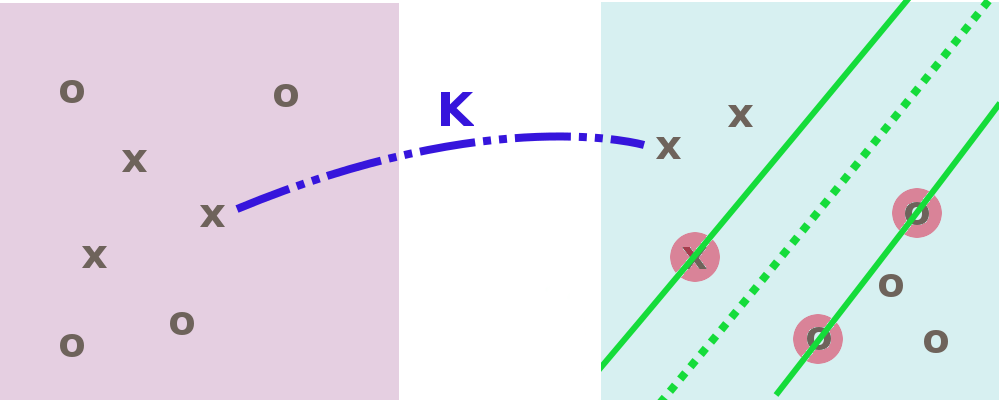
\includegraphics[width=0.8\textwidth]{svm_graph}
		\label{figure:svm_graph}		
	\end{figure}
	
	\subsection{Design}
		
	\subsubsection{Linear Classification}
	SVM uses the so-called ``Kernel trick" to separate points from different classes.
	\Cref{figure:svm_graph} shows two spaces with vectors of different classes.
	%Suppose that the vectors represented with x's are composite numbers and the o's are primes. 
	Since we cannot use a straight line (or hyperplane in higher dimensions) to separate the two classes in the left space, we use a nonlinear transformation $K$ (commonly referred to as a Kernel function) to map these vectors into a higher dimensional space where the two classes are separable. Of course, this trick requires that we first assume that such a function exists.
	
	\subsubsection{Nonlinear Transformations}
	The following functions are commonly used for the nonlinear transformation $K$. \cite{scikit-learn}
	
	\begin{itemize}
		\item linear: $\langle x, x^\prime \rangle$.
		\item polynomial: $( \gamma \langle x, x^\prime + r \rangle^d$, with $\gamma, r \in \R$ and $d \in \N$.
		\item rbf: $\langle x, x^\prime \rangle$, where $\gamma \in \R$ with $\gamma > 0$.
		\item sigmoid: $\langle x, x^\prime \rangle$, with $r \in \R$.
	\end{itemize}

	\subsubsection{Widest Street Approach}
	Once the classes are linearly separable, we take the ``widest street approach" \cite{mit} to construct the optimal hyperplane.
	This means choosing the hyperplane that creates the largest margin possible between vectors of different classes.
	In general, ``the larger the margin the lower the generalization error." \cite{scikit-learn}
	SVM uses a Lagrangian method for constrained optimization in order to maximize the margin width.
	%Let $S \subset \R^n$ be the space on the right-hand side of \cref{figure:svm_graph}, and let $\vec{w} \in S$ be a vector that is orthogonal to the hyperplane by represented the dashed line.	
	
%	\begin{definition}[Support Vector Machine]
%		A Support Vector Machine (SVM) is a learning system that uses a hypothesis space of linear functions in a high dimensional feature space, trained with a learning algorithm from optimisation theory that implements a learning bias derived from statistical learning theory.\cite{christianini}
%	\end{definition}
%	
%	
%	\begin{itemize}
%		\item target function --- underlying function that maps inputs to outputs (if it exists)
%		\item solution --- estimate of the target function by learning algorithm (also called the decision function in classification algorithms)
%		\item hypothesis space --- a set or class of candidate solutions (known as hypotheses)
%		\item learning algorithm --- uses training data to select a hypothesis 
%		\item features --- the quantities used to describe the data
%		\item attributes --- original quantities from data
%	\end{itemize}
%	
		
%	\subsection{Vector Spaces}
%
%	\begin{definition}[Hyperplane]
%		Let $a_1,a_2,\ldots,a_n$ be scalars not all equal to 0. Then the set $S$ consisting of all vectors $$x = \begin{pmatrix} x_1 \\ x_2 \\ \vdots \\ x_n \end{pmatrix} \in \R^n$$ such that $a_1x_1 + a_2x_2 + \cdots + a_nx_n = c$ for a constant $c$ is a subspace of $\R^n$ called a \textbf{hyperplane}.\cite{mathworld:hyperplane}
%	\end{definition}
%	
%	\subsection{Inner Product Spaces}
%	
%	\begin{definition}[Gram matrix]
%		Given a set $V$ of $m$ vectors (points in $\R^m$), the \textbf{Gram matrix} $G$ is the matrix of all possible inner products of $V$, i.e., $$ g_{ij}  = v_i^Tb_j, $$ where $A^T$ denotes the transpose. The Gram matrix determines the vectors $v_i$ up to isometry. \cite{mathworld:gram_matrix}
%	\end{definition}
%	
%	\subsubsection{Hilbert Spaces}
%	
%	\begin{definition}[Hilbert Space]
%		A \textbf{Hilbert space} is a vector space $H$ with an inner product $\langle f,g \rangle$ such that the norm defined by $$ |f| = \sqrt{\langle f,f \rangle} $$ turns $H$ into a complete metric space. If the metric defined by the norm is not complete, then H is instead known as an inner product space. \cite{mathworld:hilbert_space}
%	\end{definition}
%	
%	\subsection{Operators, Eigenvalues and Eigenvectors}
%	
%	\subsection{Kernel Induced Feature Spaces} % christianini chapters 2 and 3
%	
%	``Project the data into a higher dimensional feature space to increase the computational power of the linear learning machines." \cite{christianini}
%	
%	\begin{definition}[Kernel \cite{christianini}]\label{definition:kernel}
%		A kernel is a function $K$, such that for all $x, z \in X$
%		$$ K(x,z) = (\phi(x) \cdot \phi(z)),$$
%		where $\phi$ is a mapping from $X$ to an (inner product) feature space $F$. 
%	\end{definition}
%	
%	\begin{example}
%		Map input space into new space.
%	\end{example}
%	
%	``not scale invariant, so it is highly recommended to scale your data. For example, scale each attribute on the input vector $X$ to [0,1] or [-1,+1], or standardize it to have mean 0 and variance 1."
%	
	
	
	
	
	%\subsection{Learning Bias} % christianini chapter 4
	
	%\subsection{Learning Algorithm} % christianini chapters 5 and 7
	
	%\subsection{Cononical Hyperplane}
	
	%\subsection{Lagrangian Optimization}
	
	% ==========================================================================
	% Method
	% ==========================================================================	
		
	\subsection{Method}\label{method}
	We used scikit-learn's implementation of SVM.
	This choice was made due to scikit-learn's popularity and ease of use.
	We arbitrarily chose the rbf function as the nonlinear transformation $K$.
	\footnote{
		Scikit-learn has four built-in functions: linear, polynomial, rbf, and sigmoid.	
		We believe that this classification problem requires a custom function.
		However, much more research is needed in order to find a function that can separate the primes from the composites.
	}			
	%We will attempt to classify integers between 2 and 1000 (inclusive).
	
	\subsubsection{Input Vectors}
	
	We arbitrarily chose 1000 as the largest integer, and so we only attempted to classify integers between 2 and 1000 (inclusive). 
	Since SVM requires vector inputs, we will use the digits of the base-b representation of an integer as the entries of its input vector. Since SVM is scale invariant \cite{scikit-learn}, we also scaled each input vector to $[-1,1]$.

	\begin{example}
		Suppose that we are using base 3. Then $(5,2)$ is the input vector for $32 \in \Z$. Likewise, the integers $153$ and $1000$ are represented by $(4,1,3)$ and $(4,3,4,4)$, respectively. Since 1000 is the largest integer that we are interesting in, $(4,3,4,4)$ is the longest vector in this input vector space. 
	\end{example}
	
	\begin{figure}
		\caption{Base 32 representations of integers between 2 and 1000 (inclusive).}		
		\centering
			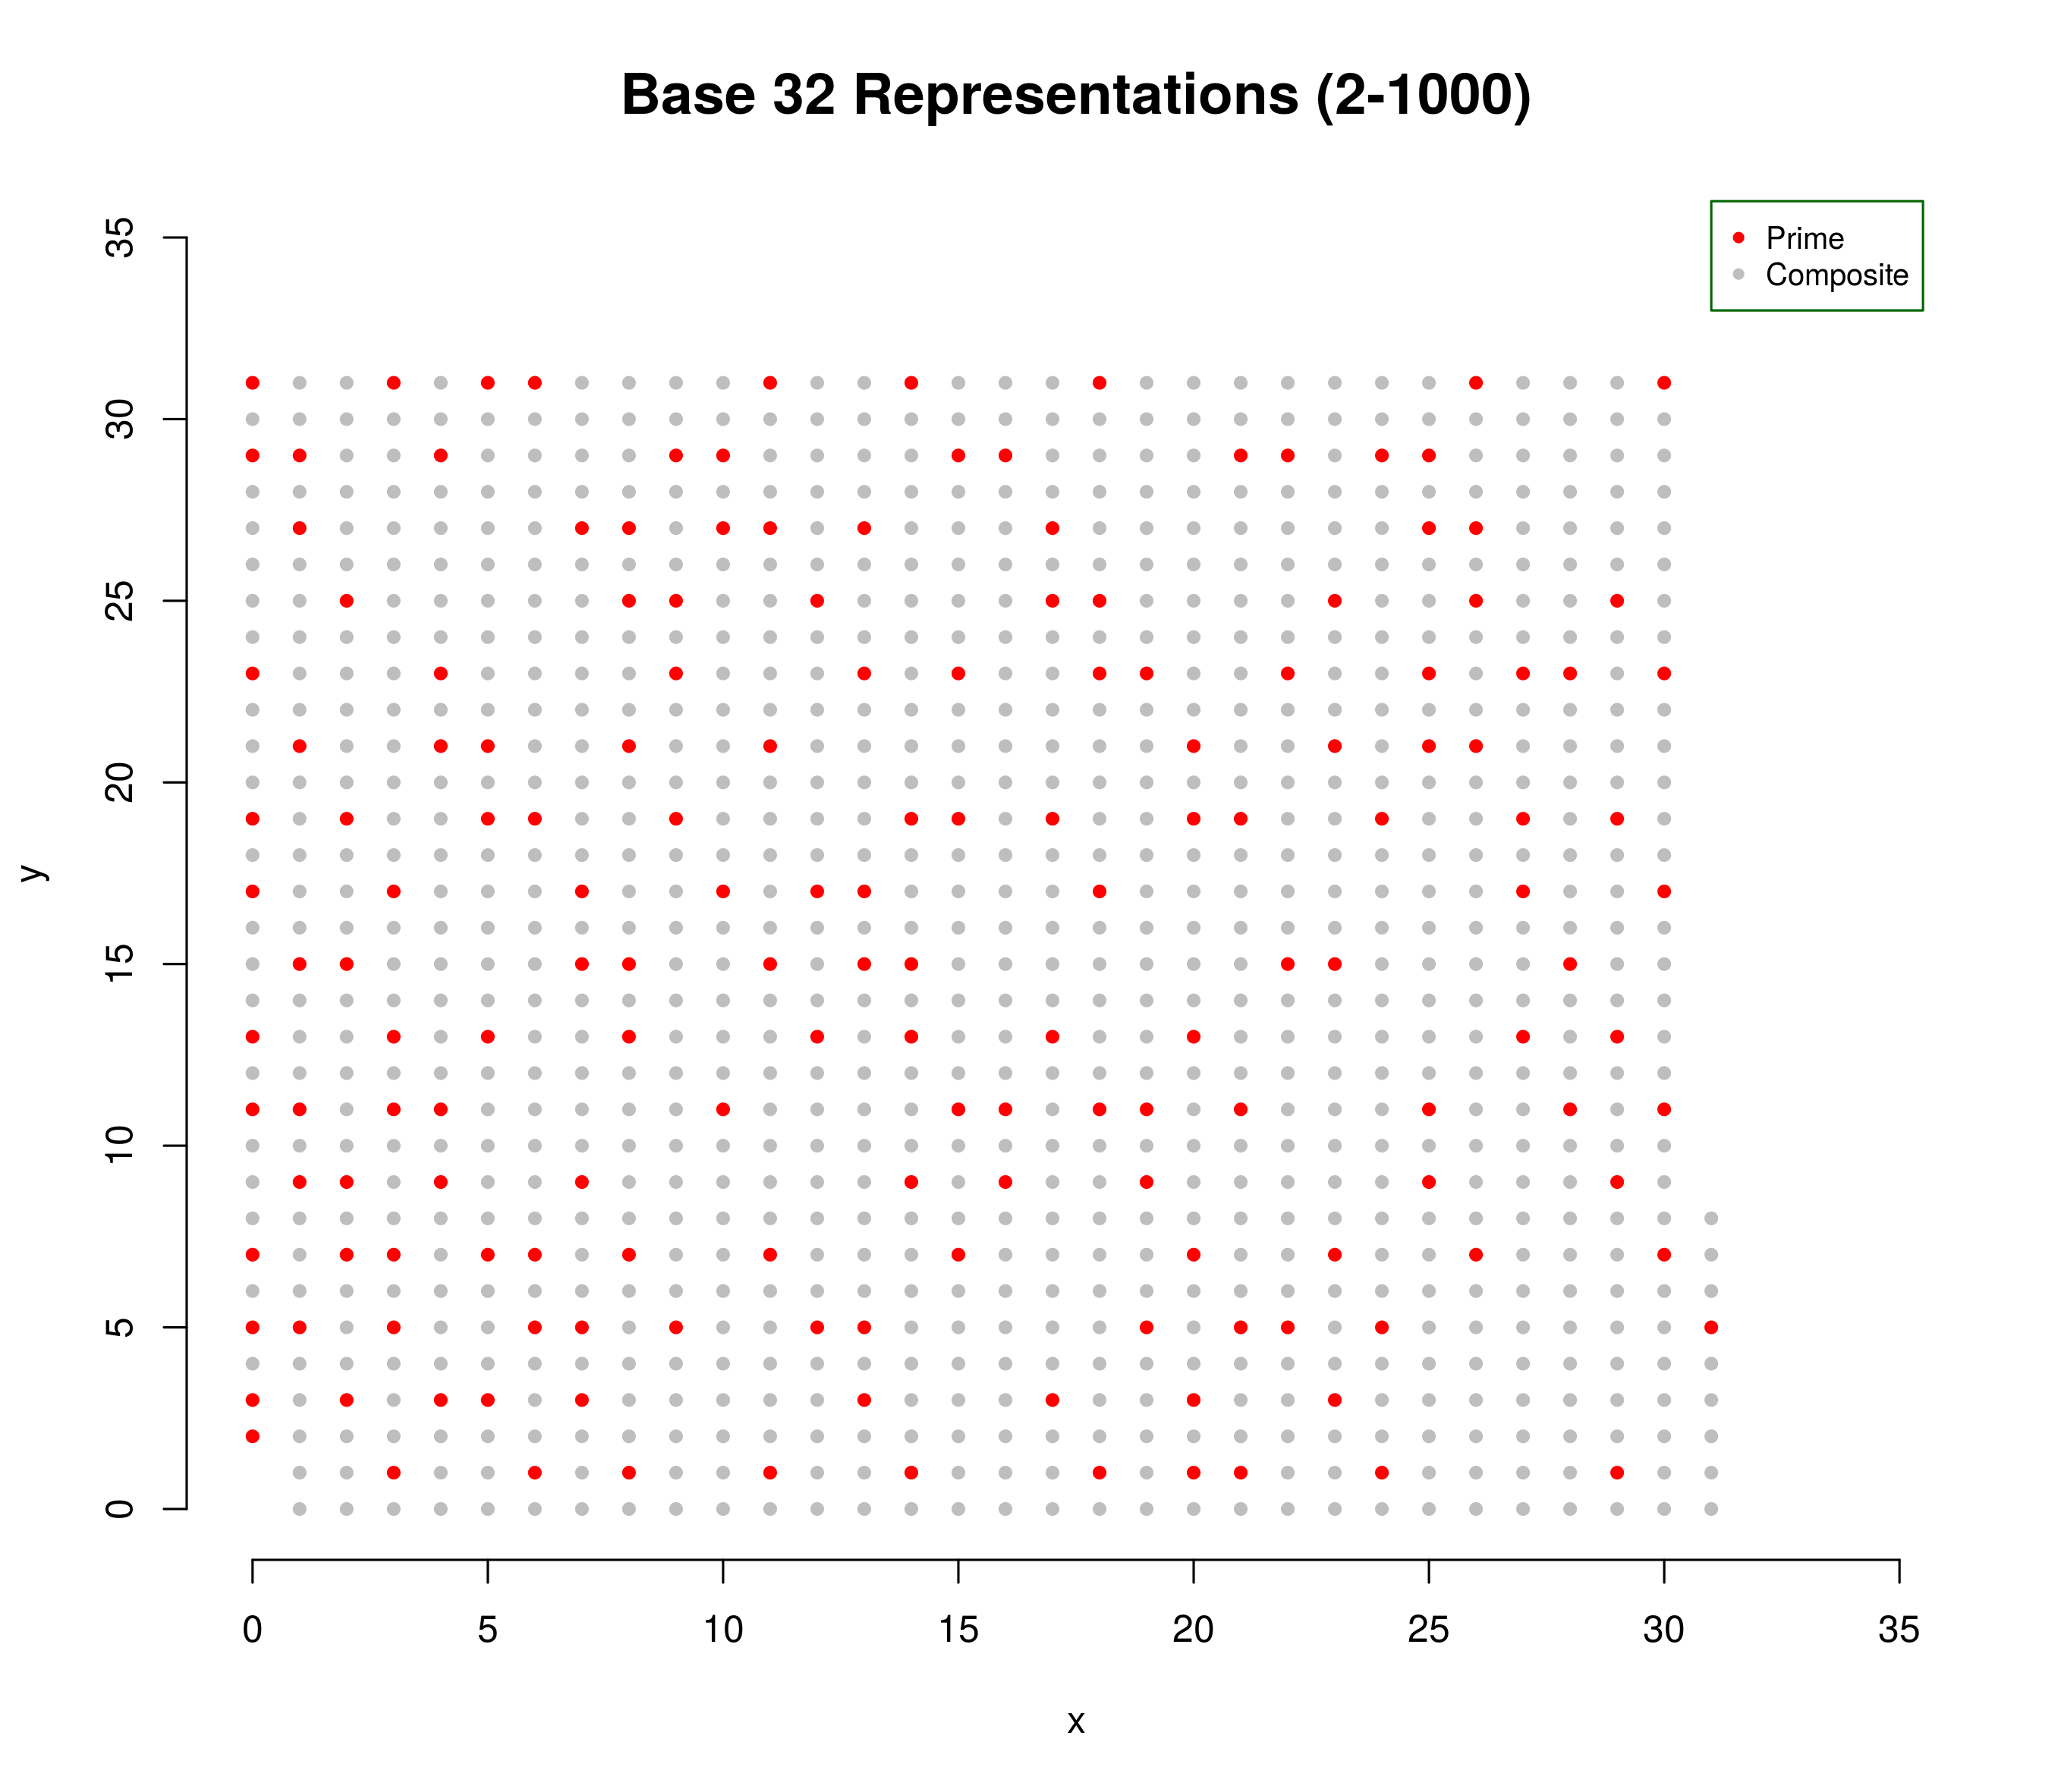
\includegraphics[width=0.7\textwidth]{base_32}
		\label{figure:base_32}
	\end{figure}

	
	%\subsubsection{Training Data}
	
%	We will use $X \subset \R^n$ and $Y = (-1, 1)$ for binary classification. 
%	
%	\begin{definition}[Training Set]
%		A \textbf{training set} is a collection of training examples, which are also called training data. It is usually denoted by $S = \{ (x_1, y_1),(x_2, y_2),\ldots, (x_n, y_n)\} \subset X \times Y$, where $n$ is the number of examples. We refer to $x_i$ as examples or instances and $y_i$ as their labels.\cite{christianini}
%	\end{definition}
	
	%\subsubsection{Base-b Representations}	
	
%	\begin{theorem}[Well Ordering Principle]\label{theorem:well_ordering_principle}
%		Every nonempty set of positive integers contains a smallest member. \cite{mathworld:well_ordering_principle}
%	\end{theorem}
%	
%	\begin{proof}
%		Let $A \subseteq \Z^+ : A \neq \emptyset$. Assume for the sake of contradiction that $A$ does not have a smallest member. Then $1 \not\in A$ since $1 \leq n$ for all $n \in \Z^+$. Now we assume positive integers $1, 2, \ldots, k \not\in A$. Then $k + 1 \not\in A$ since $k + 1$ would be the smallest member of $A$. Thus, by strong induction $A = \emptyset$, a contradiction. Therefore, $A$ must contain a smallest member.
%	\end{proof}
%	
%	\begin{theorem}[The Division Algorithm]\label{theorem:division_algorithm}
%		Let $a, b \in \Z : b > 0$. Then there exist unique $q, r \in \Z$ such that $ a = bq + r $ and $0 \leq r < b$. \cite{pommersheim}
%	\end{theorem}	
%	
%	\begin{proof}
%		Let $a, b \in \Z : b > 0$, and let $R = \{ x \in \Z : a - xb \geq 0 \}$. First, we notice that $R \neq \emptyset$ for if $a \leq 0$ and $x = a$ then $a - ab = a(1-b) \geq 0$, and if $a > 0$ and $x = 0$ then $a - 0 \cdot b \geq 0$. 
%		
%		Thus, by \cref{theorem:well_ordering_principle}, $R$ contains a smallest member, which we will call $r$. Hence, $\exists q \in \Z : r = a - qb \geq 0$. Now suppose for the sake of contradiction that $r \geq b$. 
%		Then $r = b + n \geq 0$ for some $n \in \Z: n \geq 0$. Hence, $r = b + n = a - qb$ or $n = a - qb - b = a - (q + 1)b \in R$. But $n = a - (q + 1)b < a - ab = r$ is impossible since $r$ is the smallest member of $R$. So, it must be that $r < b$. Therefore, we have found $q, r \in \Z$ such that $ a = bq + r $ and $0 \leq r < b$.
%		
%		To complete the proof, we must show that $q$ and $r$ are unique. So, we let $q^\prime, r^\prime \in \Z$ and assume $a = q^\prime b + r^\prime$ such that $0 \leq r^\prime < b$. Thus, $a = qb - r = q^\prime b + r^\prime$. In other words,  $r - r^\prime = q^\prime b - qb $ or $r - r^\prime = b (q^\prime - q)$. Without loss of generality, we may assume that $r^\prime \leq r$ such that $0 \leq r - r^\prime \leq r < b$. Therefore, $r - r^\prime$ must be a nonnegative multiple of $b$, such as $0, b, 2b, 3b, \ldots$, but $r - r^\prime < b$ implies that $r - r^\prime = 0$ or $r = r^\prime$. Also, since $b > 0$, $r - r^\prime = 0 = b (q^\prime - q) = b \cdot 0$. Thus, $q^\prime - q = 0$ or $q^\prime = q$. Therefore, $q$ and $r$ are unique.
%		
%		%Furthermore, we know $0 \leq q^\prime - q$ because $0 \leq r - r^\prime$ and $0 < b$.
%		
%		%By \cref{definition:divisibility}, $r - r^\prime = b (q^\prime - q) $ if and only if $b | r - r^\prime$. This implies $b \leq r - r^\prime$ according to \cref{lemma:divisibility}. 
%		% Since $r - r^\prime < 0$ or $r^\prime > r$ contradicts the assumption that $r^\prime \leq r$, we know $r - r^\prime = 0$ or $r^\prime = r$. It follows that $r - r^\prime = 0 = b (q^\prime - q)$ if and only if $q^\prime - q = 0$ or $q^\prime = q$, since $b > 0$. Therefore, $q$ and $r$ are unique. 
%	\end{proof}
	
	
	%\subsection{Base-b Representations}
	
%	\begin{cor}
%		Let $b \in \Z : b \geq 2$. Then every $N \in \Z : N > 0$ can be expressed uniquely in the form $N = a_kb^k + a_{k-1}b^{b-1} + \cdots + a_1 b + a_0$, where $a_0, a_1, \ldots, a_k$ are nonnegative integers less than $b$, $a_k \neq 0$, and $k \geq 0$. \cite{koshy}
%	\end{cor}
	
	%\subsection{Operations in Nondecimals Bases}
	
	
	
	\subsubsection{Finding the Best Parameters}
	
	We used trial and error to find the base-b representation and SVM parameters that would maximize the mean accuracy of the algorithm.
	We experimented with base-b representations ranging from 2 to 500.
	We also considered different combinations of the following SVM parameters:
	\begin{itemize}
		\item class weight for input vectors that represent prime numbers, and
		\item penalty parameter $C$.
	\end{itemize}
	Usually, each class of input vectors has the same weight.
	However, there are only 168 primes between 2 and 1000. 
	Thus, we tried different values for weight of the prime class.
	The penalty parameter $C$ is the upper bound of the Lagrangian multipliers used in the optimization problem describe above.
	For each of these values, we tried values between 1 and 100.
	
	\subsubsection{Results}
	We refer to a particular combination of parameters as a model.
	The best models had a mean accuracy\footnote{Accuracy is the function $f: \N^2 \to \R \cap [0,1]$ defined by $f(a, b) := \frac{a}{a + b}$, where $a$ is the number of correct predictions and $b$ is the number of incorrect predictions.} equal to 0.86. Interestingly, all of these models used base 6 representations and a prime class weight of 2, with the penalty parameter $C$ ranging from 3.2 to 4.9 (see \cref{appendix:best_params}).
	
	A mean accuracy of 0.86 seems like a promising result. However, \cref{figure:complexity} shows that a large number of models achieved a mean accuracy greater than 0.8 regardless of the parameters used (notice the thick line near the top).
	This lack of correlation is alarming.
	Since 82.8 percent of the integers between 2 and 1000 are composite, we suspect that the best models were simply classifying every integer as composite. Conversely, many models classified every integer as prime (notice the thick line near the bottom).
	
	\begin{figure}
		\centering
			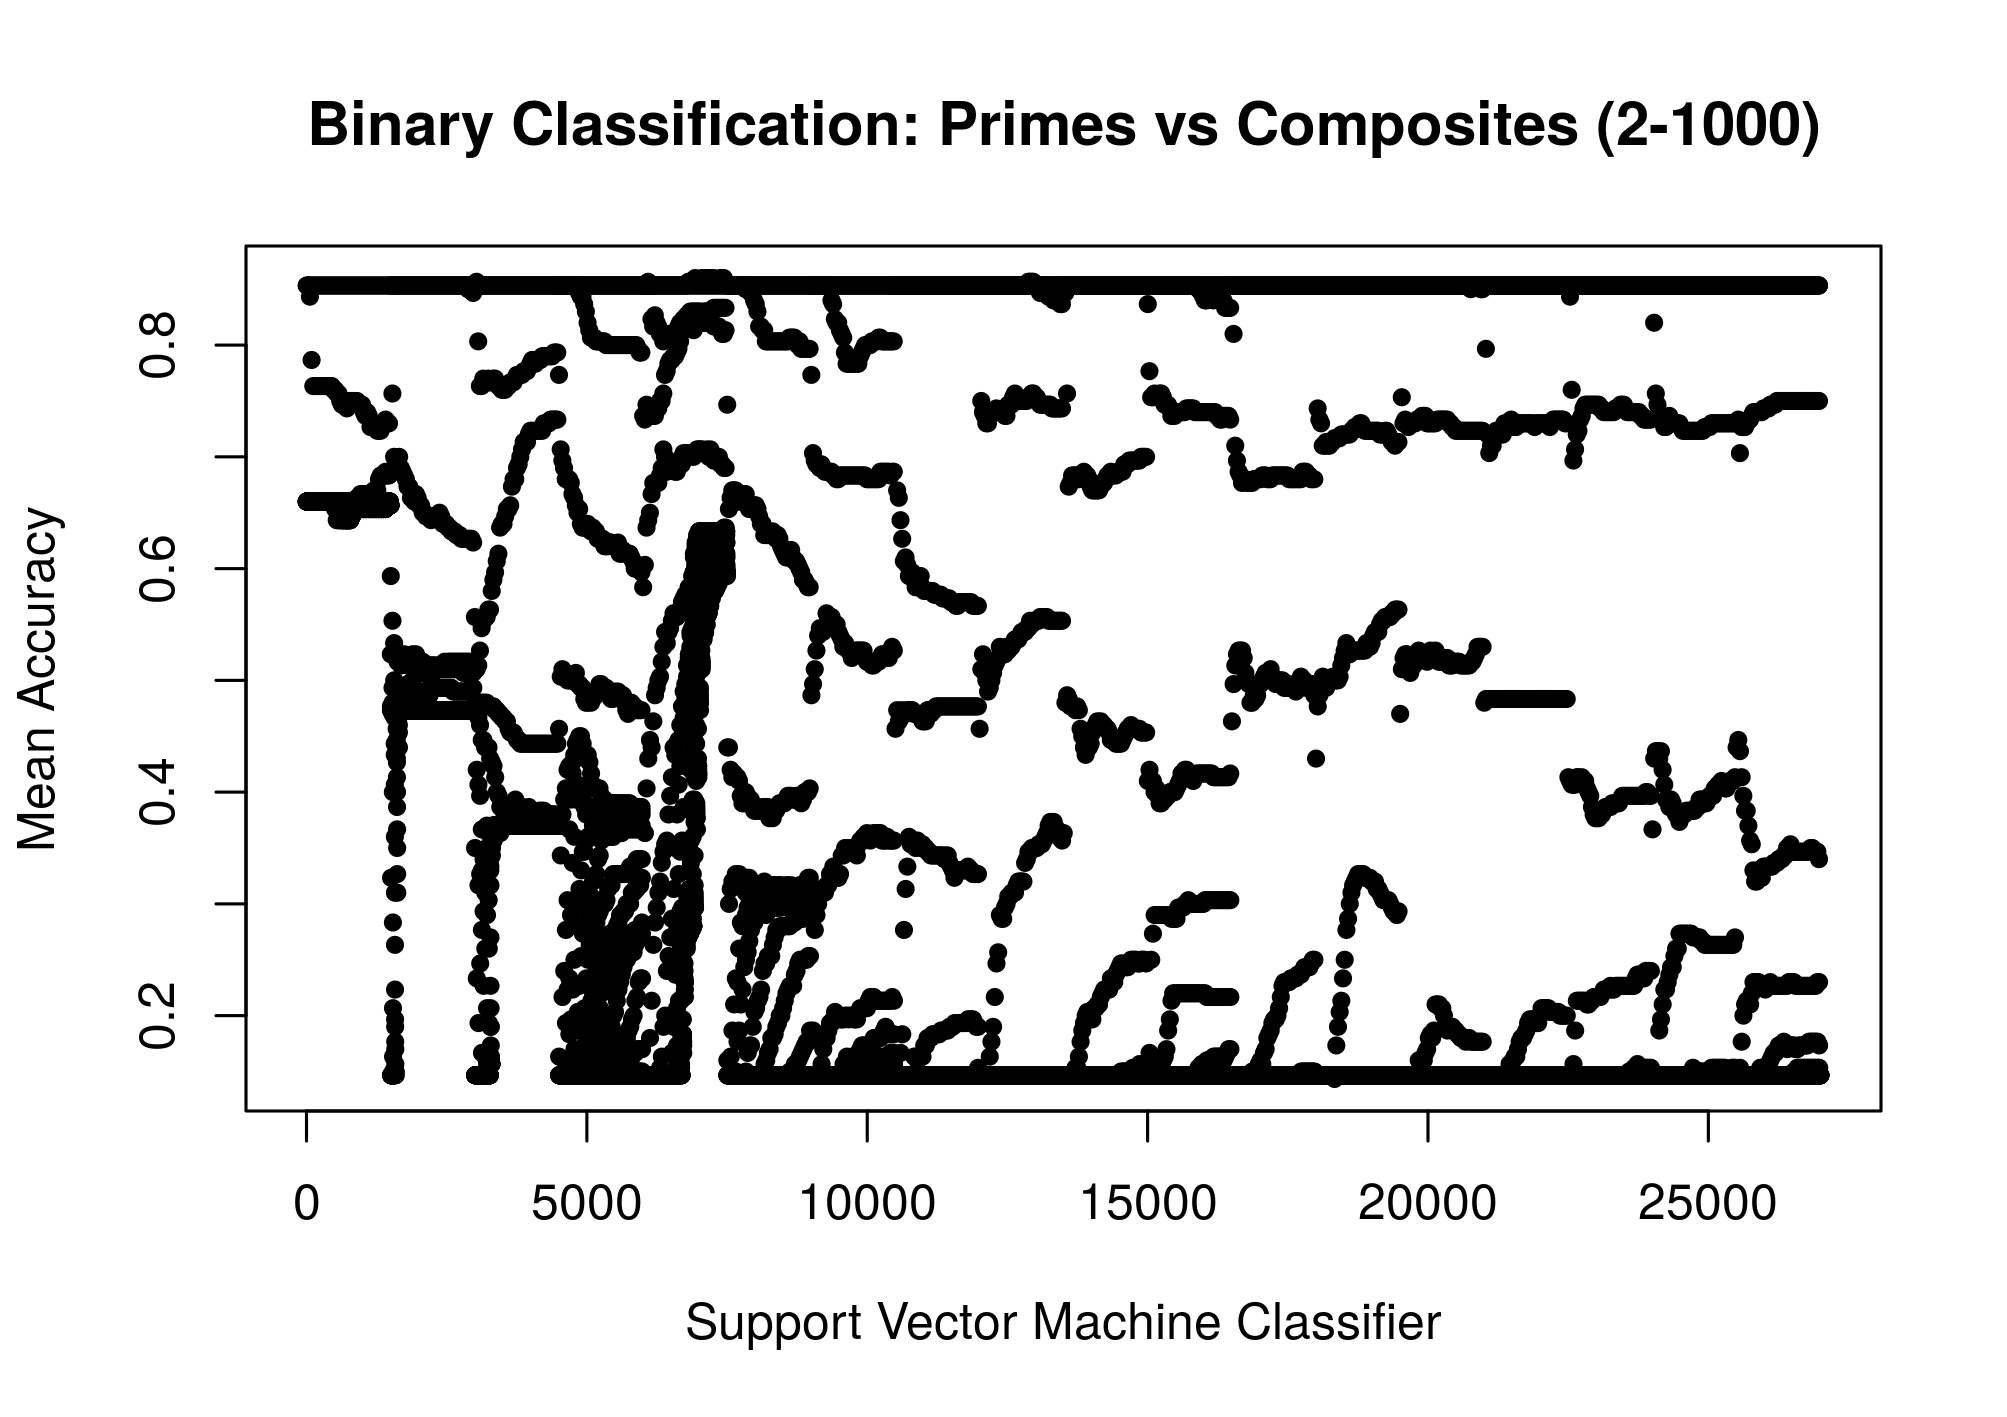
\includegraphics[width=0.8\textwidth]{complete}
		\caption{Complexity vs Mean Accuracy}
		\label{figure:complexity}
	\end{figure}

	% ==========================================================================
	% Conclusion
	% ==========================================================================	
		
	\section{Conclusion}\label{conclusions}
	We conjecture that SVM's performance would improve and possibly exceed common tests for compositeness with the right transformation $K$. 
	However, if it exists, finding such a function that maps integers into a space where composite numbers and primes are separable will require much more research.
	Nevertheless, it is a worthwhile endeavor for number theorists and cryptologists alike.  
	Pierre de Fermat first stated Fermat's Little Theorem nearly 400 years ago in a letter dated October 18, 1640 \cite{wiki:fermats_little_theorem}. 
	Remarkably, it remains at the heart of a test for compositeness that still outperforms modern machine learning algorithms! For good reason, programming languages like Maple and Wolfram implement the Miller-Rabin test.
	
	
	\clearpage
	
	
	\begin{appendix}
	\section{Miller-Rabin Test Results for 169}\label{appendix:results_for_169}
	
	The Miller-Rabin test was performed with each nonzero $\bar{a} \in 169$, starting with $\bar{1}$ and ending with $\overline{168}$.
	Of these, 156 are Miller-Rabin witnesses to the compositeness of 169, namely, 
	
	\begin{seqsplit}				
	2, 3, 4, 5, 6, 7, 8, 9, 10, 11, 12, 13, 14, 15, 16, 17, 18, 20, 21, 24, 25, 26, 27, 28, 29, 30, 31, 32, 33, 34, 35, 36, 37, 38, 39, 40, 41, 42, 43, 44, 45, 46, 47, 48, 49, 50, 51, 52, 53, 54, 55, 56, 57, 58, 59, 60, 61, 62, 63, 64, 65, 66, 67, 68, 69, 71, 72, 73, 74, 75, 76, 77, 78, 79, 81, 82, 83, 84, 85, 86, 87, 88, 90, 91, 92, 93, 94, 95, 96, 97, 98, 100, 101, 102, 103, 104, 105, 106, 107, 108, 109, 110, 111, 112, 113, 114, 115, 116, 117, 118, 119, 120, 121, 122, 123, 124, 125, 126, 127, 128, 129, 130, 131, 132, 133, 134, 135, 136, 137, 138, 139, 140, 141, 142, 143, 144, 145, 148, 149, 151, 152, 153, 154, 155, 156, 157, 158, 159, 160, 161, 162, 163, 164, 165, 166, 167.
	\end{seqsplit}

	Thus, more than 9 out of 10 elements in $\Z_{169}$ are witnesses.
	This illustrates the effectiveness of the Miller-Rabin test. 
	
	\section{Finding the Exponents}\label{appendix:finding_the_exponents}
	The most difficult step in the Miller-Rabin test for compositeness is finding the exponents. 
	However, the following code snippet demonstrates how easily this can be done in Python.
	\begin{lstlisting}[frame=single]
	# choose a and initialize n
	a, n = 154320140719312, 1
	# compute first exmponent
	exp = a / pow(2, n)
	# while 2 divides the expoenent
	while exp % 1 == 0:
	# print result
	print(exp)
	# increment n
	n = n + 1
	# compute next exponent
	exp = a / pow(2, n)
	\end{lstlisting}
	
	\newpage
	
	\section{Best Parameters}\label{appendix:best_params}
	
	\begin{figure}[h!]
		\caption{Mean accuracy converged to smallest value for bases greater than 15.}
		\centering
			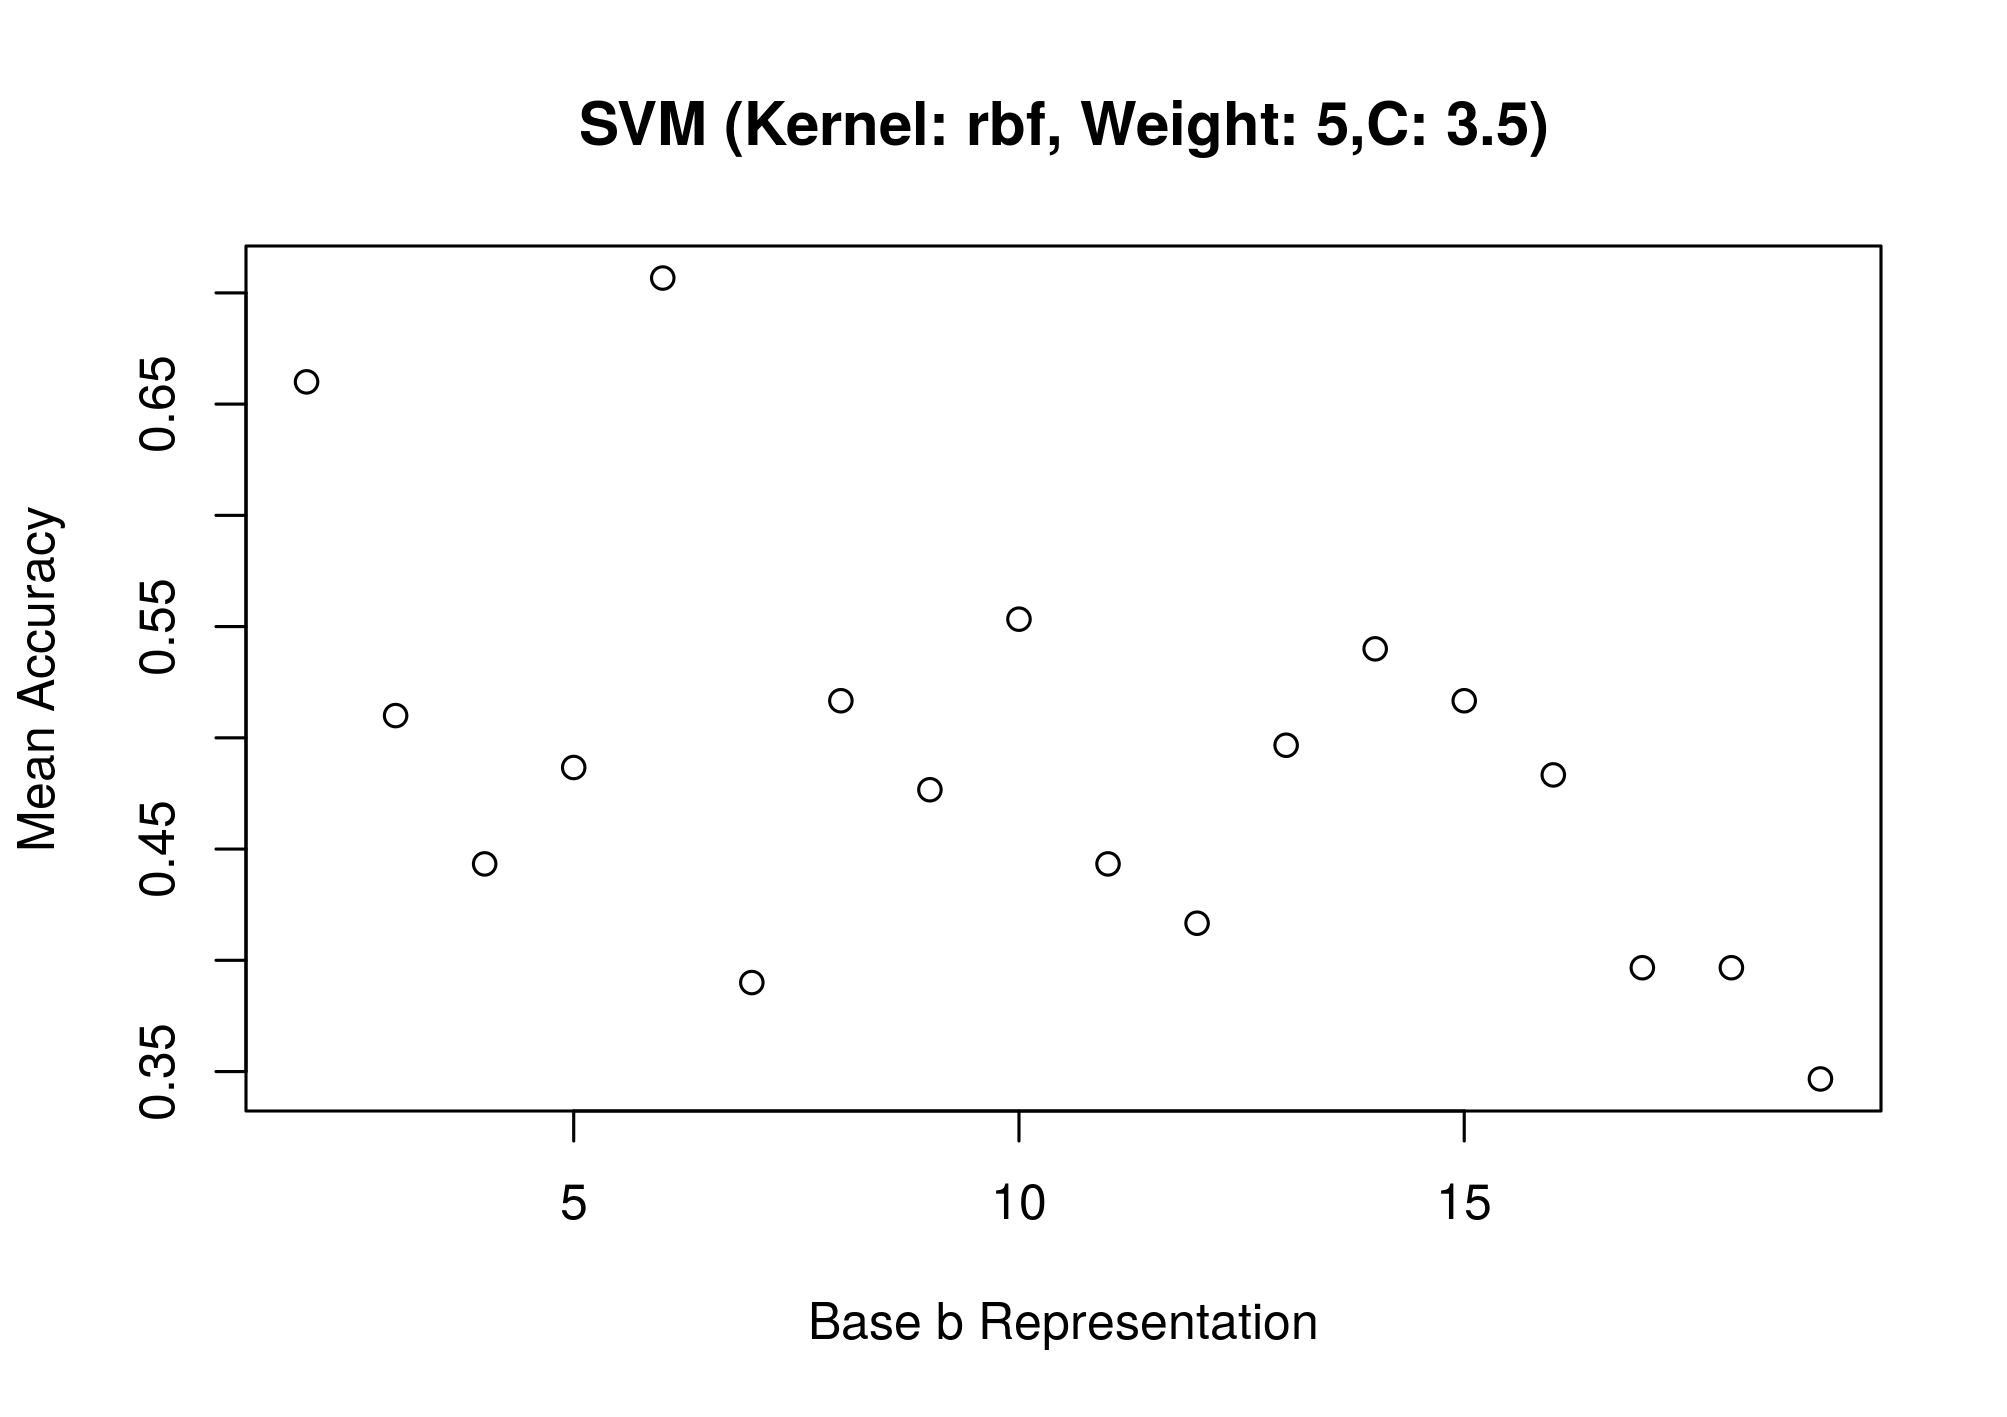
\includegraphics[width=0.7\textwidth]{base_demo}
	\end{figure}

	\begin{figure}[h!]
		\caption{The best prime class weights were less than 3.}
		\centering
			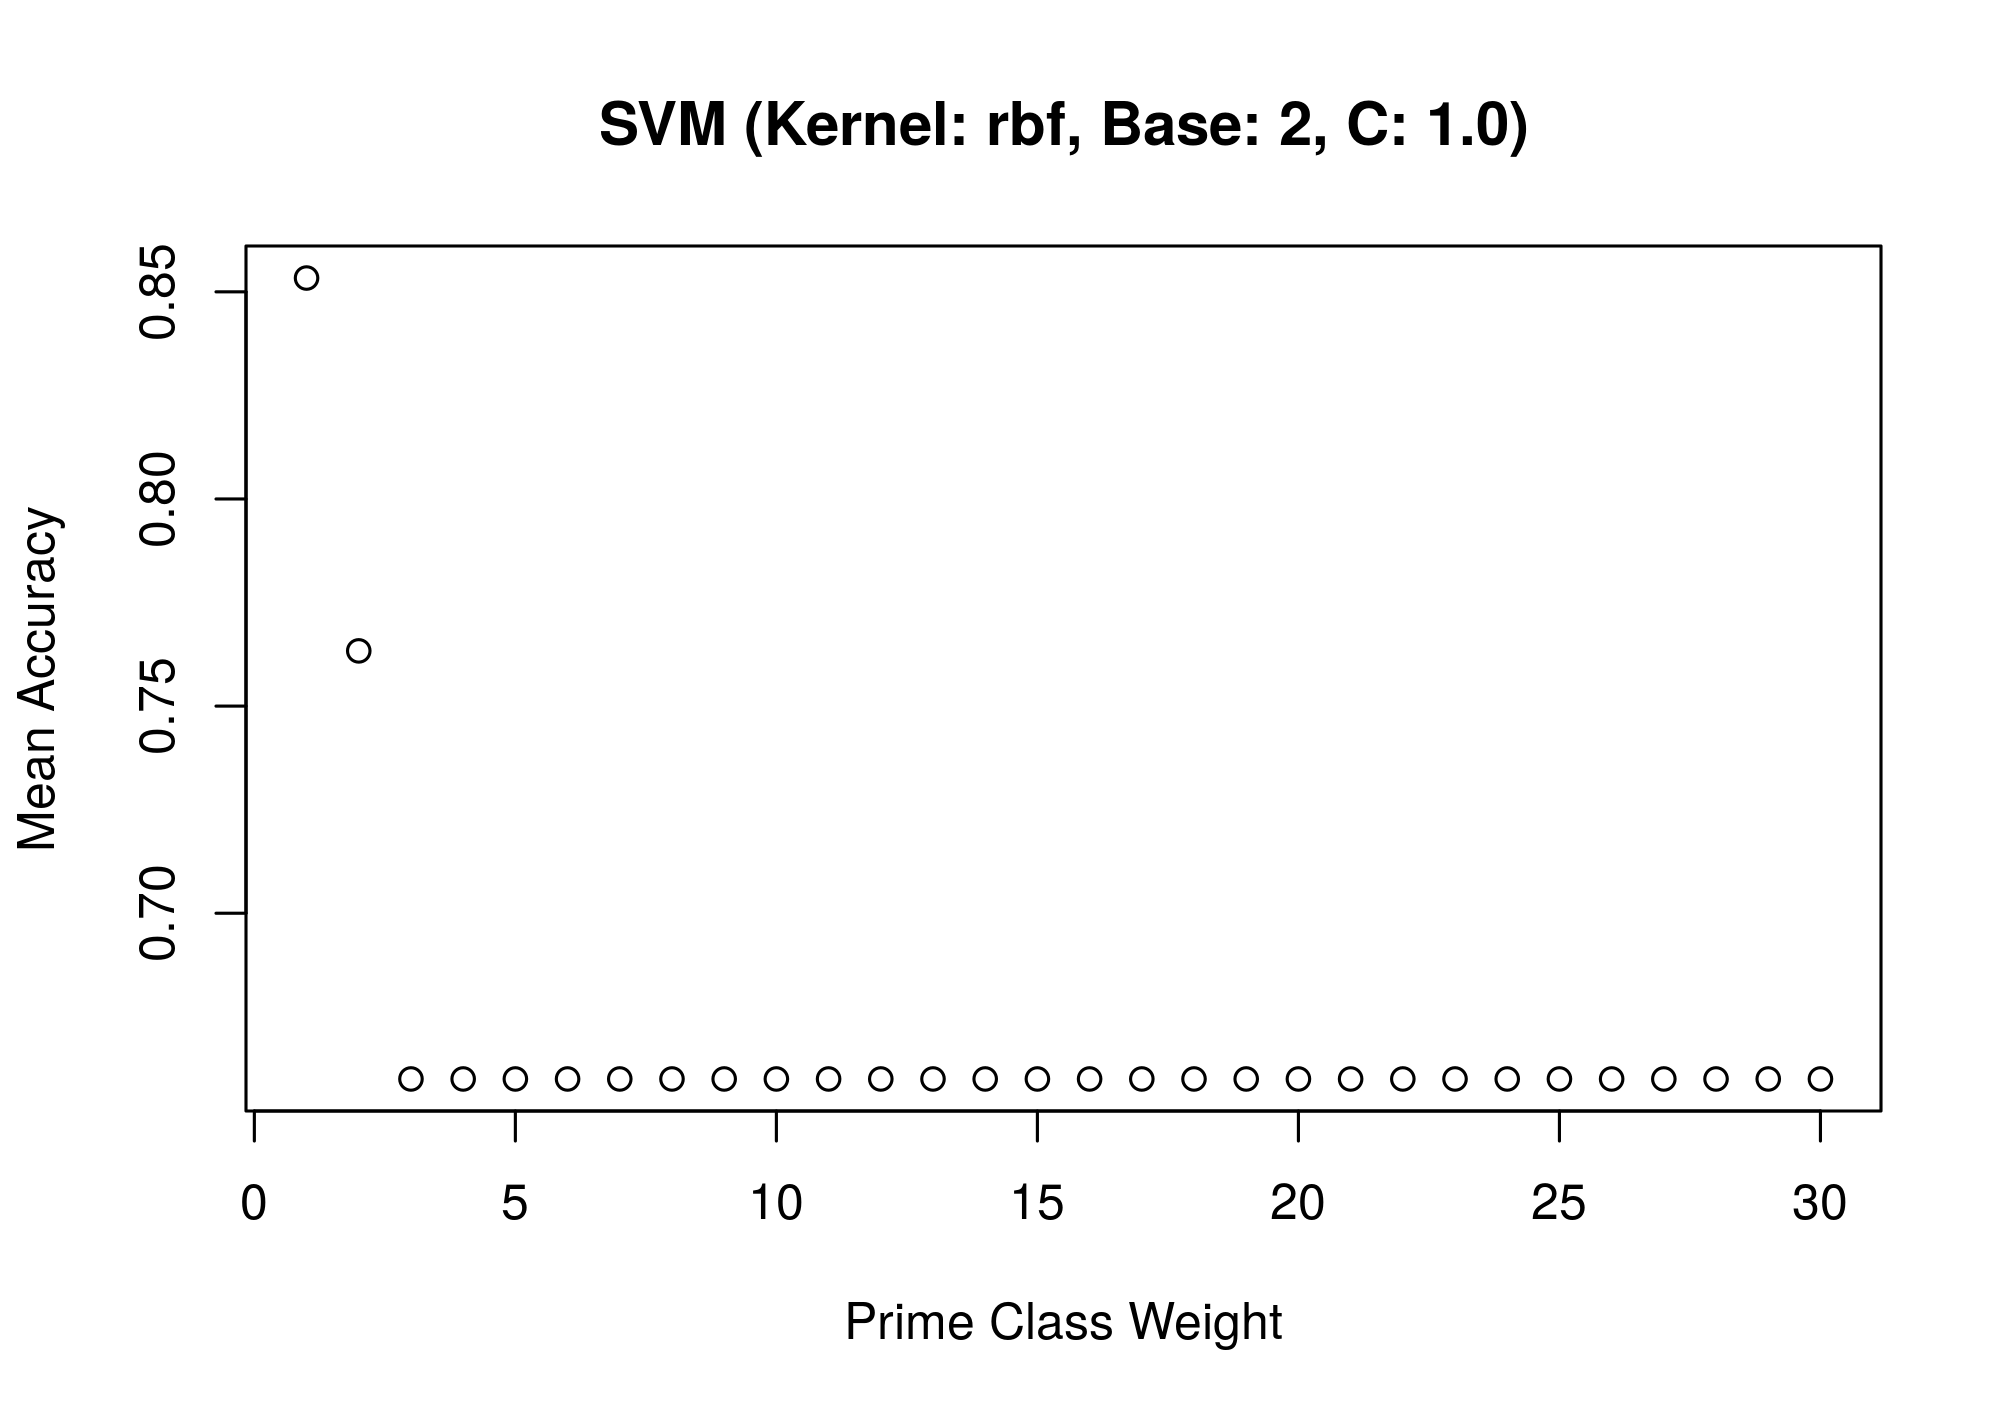
\includegraphics[width=0.7\textwidth]{weight_demo}
	\end{figure}
	
	\begin{figure}[h!]
		\caption{Models with penalty parameters $C$ between 3 and 5 had the greatest mean accuracy.}
		\centering
			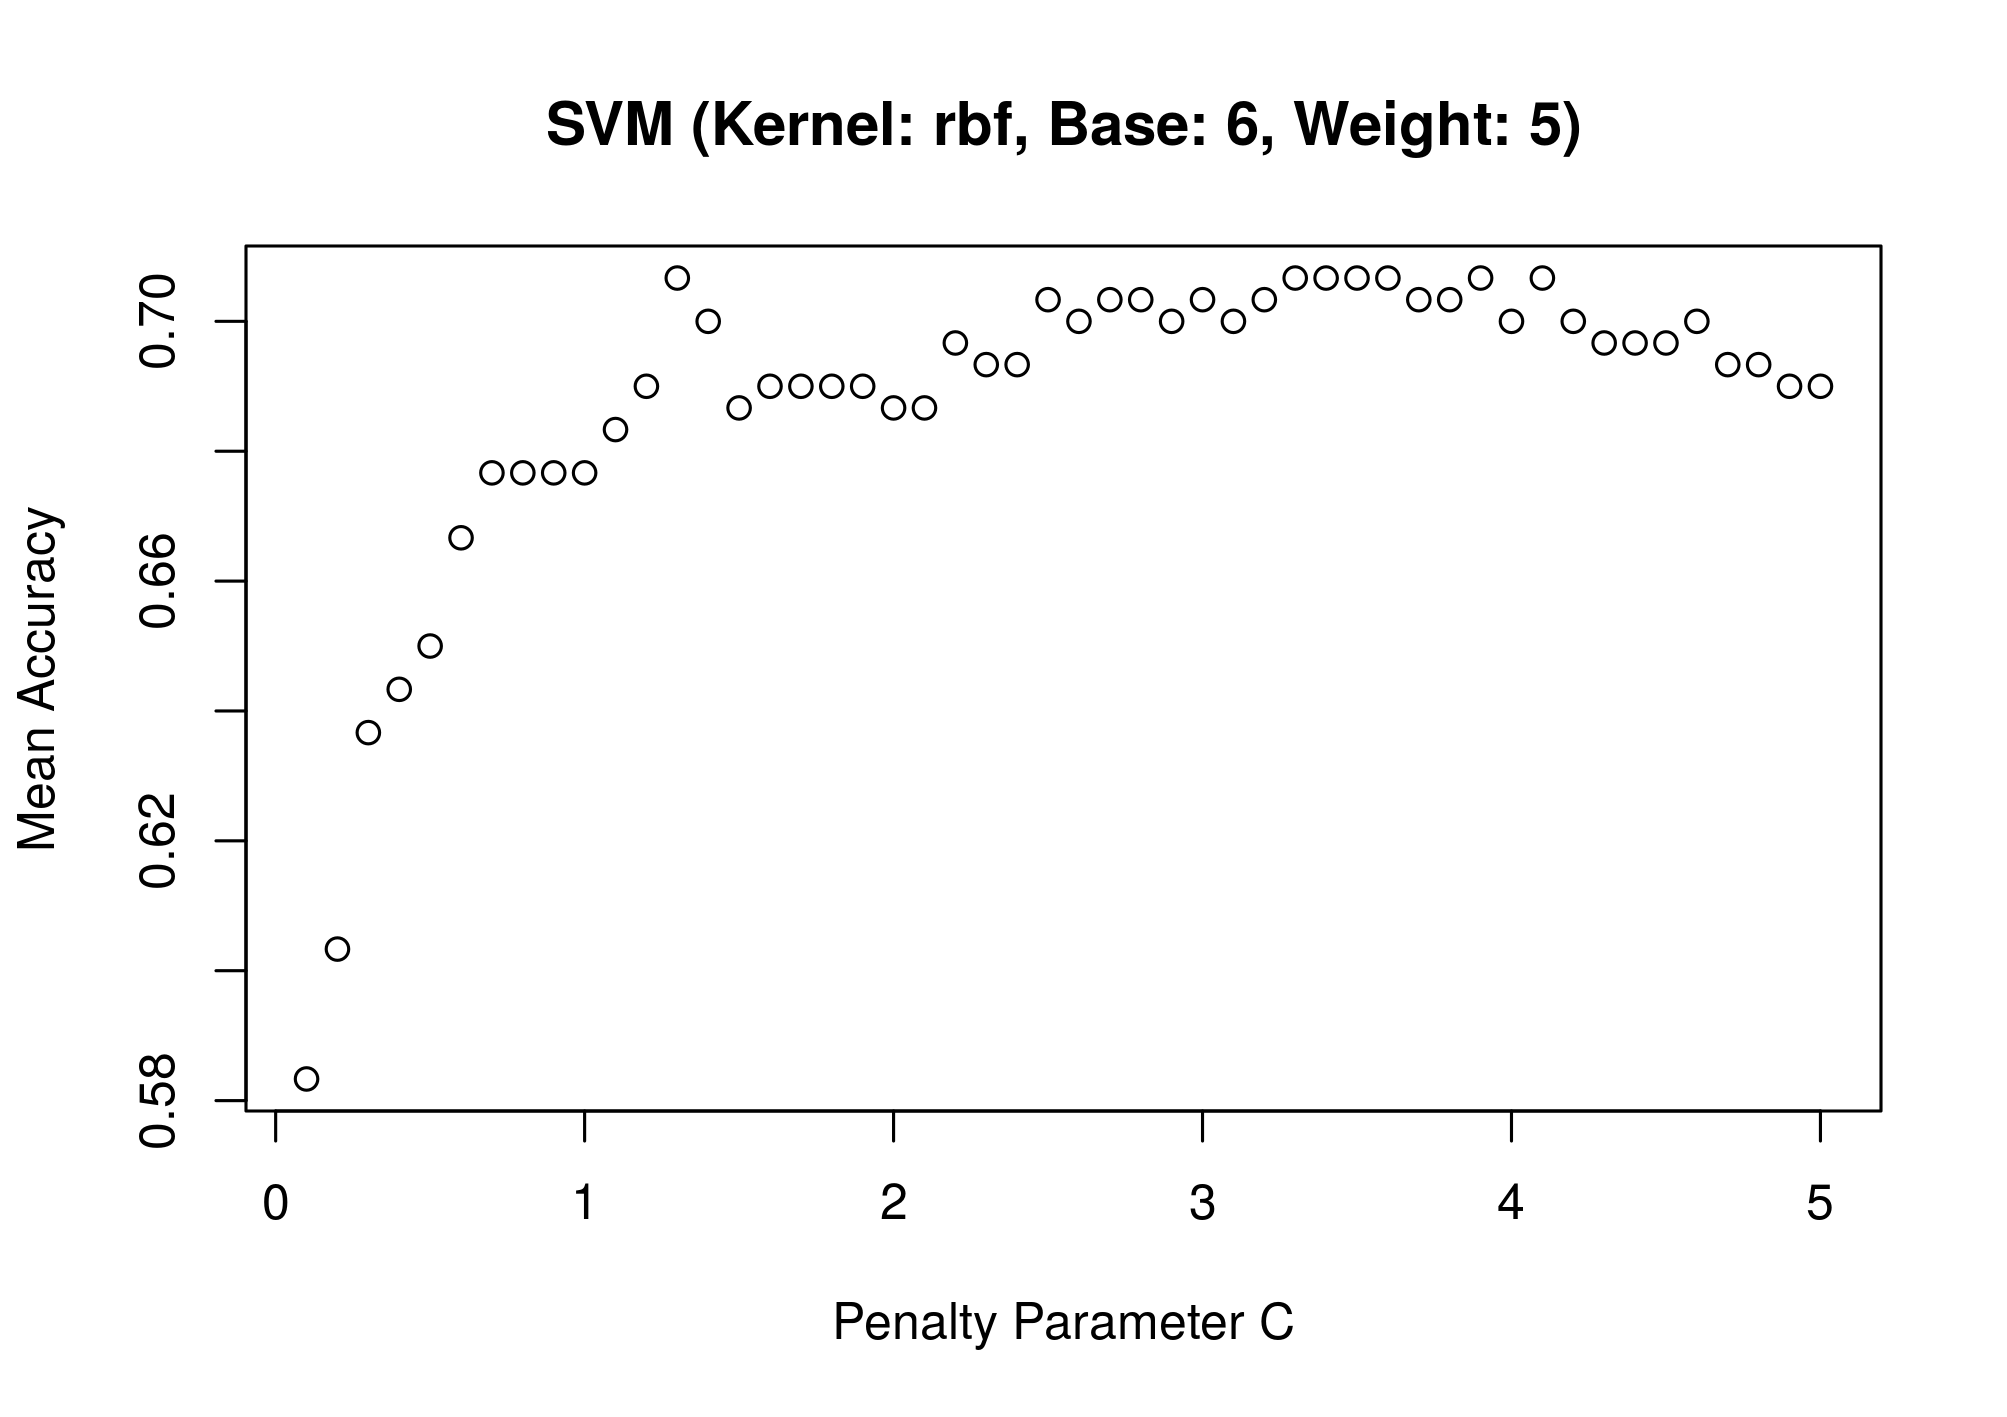
\includegraphics[width=0.7\textwidth]{c_demo}
	\end{figure}	
	
	\newpage	
%	\begin{seqsplit}
%	1, 19, 22, 23, 70, 80, 89, 99, 146, 147, 150, 168
%	\end{seqsplit}

		
%	\section{Implementation of Fermat's Test}
%	
%	\begin{lstlisting}[frame=single]
%	def fermats_test(n):
%		nonwitnesses = []
%		witnesses = []
%		for a in range(1,n):
%			right_hand_side = pow(a,n-1,n)
%			if right_hand_side is 1:
%				nonwitnesses.append(a)
%			else:
%				witnesses.append(a)
%		return [nonwitnesses, witnesses]
%	\end{lstlisting}
%	
%	Between 1 and 560 (inclusive), we have 320 integers $a$ such that for $\bar{a} \in \Z_{561}$, we have $\bar{a}^{650} = \bar{1}$.
%	
%	\begin{seqsplit}
%	1, 2, 4, 5, 7, 8, 10, 13, 14, 16, 19, 20, 23, 25, 26, 28, 29, 31, 32, 35, 37, 38, 40, 41, 43, 46, 47, 49, 50, 52, 53, 56, 58, 59, 61, 62, 64, 65, 67, 70, 71, 73, 74, 76, 79, 80, 82, 83, 86, 89, 91, 92, 94, 95, 97, 98, 100, 101, 103, 104, 106, 107, 109, 112, 113, 115, 116, 118, 122, 124, 125, 127, 128, 130, 131, 133, 134, 137, 139, 140, 142, 145, 146, 148, 149, 151, 152, 155, 157, 158, 160, 161, 163, 164, 166, 167, 169, 172, 173, 175, 178, 179, 181, 182, 184, 185, 188, 190, 191, 193, 194, 196, 197, 199, 200, 202, 203, 205, 206, 208, 211, 212, 214, 215, 217, 218, 223, 224, 226, 227, 229, 230, 232, 233, 235, 236, 239, 241, 244, 245, 247, 248, 250, 251, 254, 256, 257, 259, 260, 262, 263, 265, 266, 268, 269, 271, 274, 277, 278, 280, 281, 283, 284, 287, 290, 292, 293, 295, 296, 298, 299, 301, 302, 304, 305, 307, 310, 311, 313, 314, 316, 317, 320, 322, 325, 326, 328, 329, 331, 332, 334, 335, 337, 338, 343, 344, 346, 347, 349, 350, 353, 355, 356, 358, 359, 361, 362, 364, 365, 367, 368, 370, 371, 373, 376, 377, 379, 380, 382, 383, 386, 388, 389, 392, 394, 395, 397, 398, 400, 401, 403, 404, 406, 409, 410, 412, 413, 415, 416, 419, 421, 422, 424, 427, 428, 430, 431, 433, 434, 436, 437, 439, 443, 445, 446, 448, 449, 452, 454, 455, 457, 458, 460, 461, 463, 464, 466, 467, 469, 470, 472, 475, 478, 479, 481, 482, 485, 487, 488, 490, 491, 494, 496, 497, 499, 500, 502, 503, 505, 508, 509, 511, 512, 514, 515, 518, 520, 521, 523, 524, 526, 529, 530, 532, 533, 535, 536, 538, 541, 542, 545, 547, 548, 551, 553, 554, 556, 557, 559, 560
%	\end{seqsplit}
%		
%	There are 240 Fermat's witnesses to the compositeness of 561, namely all the multiples of 3, 11, 17 that are less than or equal to 560. 
%	
%	\begin{seqsplit}
%	3, 6, 9, 11, 12, 15, 17, 18, 21, 22, 24, 27, 30, 33, 34, 36, 39, 42, 44, 45, 48, 51, 54, 55, 57, 60, 63, 66, 68, 69, 72, 75, 77, 78, 81, 84, 85, 87, 88, 90, 93, 96, 99, 102, 105, 108, 110, 111, 114, 117, 119, 120, 121, 123, 126, 129, 132, 135, 136, 138, 141, 143, 144, 147, 150, 153, 154, 156, 159, 162, 165, 168, 170, 171, 174, 176, 177, 180, 183, 186, 187, 189, 192, 195, 198, 201, 204, 207, 209, 210, 213, 216, 219, 220, 221, 222, 225, 228, 231, 234, 237, 238, 240, 242, 243, 246, 249, 252, 253, 255, 258, 261, 264, 267, 270, 272, 273, 275, 276, 279, 282, 285, 286, 288, 289, 291, 294, 297, 300, 303, 306, 308, 309, 312, 315, 318, 319, 321, 323, 324, 327, 330, 333, 336, 339, 340, 341, 342, 345, 348, 351, 352, 354, 357, 360, 363, 366, 369, 372, 374, 375, 378, 381, 384, 385, 387, 390, 391, 393, 396, 399, 402, 405, 407, 408, 411, 414, 417, 418, 420, 423, 425, 426, 429, 432, 435, 438, 440, 441, 442, 444, 447, 450, 451, 453, 456, 459, 462, 465, 468, 471, 473, 474, 476, 477, 480, 483, 484, 486, 489, 492, 493, 495, 498, 501, 504, 506, 507, 510, 513, 516, 517, 519, 522, 525, 527, 528, 531, 534, 537, 539, 540, 543, 544, 546, 549, 550, 552, 555, 558
%	\end{seqsplit}
%	
%	\listoffigures
	
	\listoftables
	
	\end{appendix}
		
		
	\newpage
		
	\bibliographystyle{plain}
	\bibliography{refs.bib}
	
	

\end{document}